\documentclass[article,A4,12pt]{llncs}
\usepackage[T1]{fontenc}
\usepackage{amsmath}
\usepackage{amssymb}
\usepackage{amsfonts}
\usepackage{mathrsfs, bm}

\usepackage{graphicx}
\usepackage{tabularx}
\usepackage{subfig}
\usepackage{epsf,times}
\usepackage{color}
\usepackage{wrapfig}
\usepackage{cases}
\usepackage{multicol}

\usepackage[T1]{fontenc}
%\newcommand{\tmname}[1]{\textsc{#1}}
%\newcommand{\tmop}[1]{\ensuremath{\operatorname{#1}}}
%\newcommand{\tmsamp}[1]{\textsf{#1}}
%\newcommand{\tmtextsc}[1]{{\scshape{#1}}}
%\newcommand{\tmtextsl}[1]{{\slshape{#1}}}
%\newcommand{\tmtexttt}[1]{{\ttfamily{#1}}}

\leftmargin=0.0cm
\oddsidemargin=0.5cm
\evensidemargin=0.5cm
\topmargin=0cm
\textwidth=16.0cm
%\textheight=21.5cm
\textheight=20.0cm
\pagestyle{plain}
\setlength{\columnsep}{20pt}

\def\m{\mathbf{m}}
\def\H{\mathbf{H}}
\def\E{\mathbf{E}}
\newcommand{\vepsi}{{\varepsilon}}
\def\hnorm#1#2{\vert\,#1\,\vert_{#2}}
\newcommand{\R}{{\mathbb R}}
\newcommand{\Sph}{{\mathbb S}}
\def\x{\mathbf{x}}
\def\hvec{\overline{\mathbf{h}}}
\def\evec{\overline{\mathbf{e}}}

\newcommand{ \etal}{\mbox{\emph{et al. }}}

\newcommand\vect[1]{\mbf{#1}}
\newcommand{\mbf}[1]{\mbox{\boldmath$#1$}} 
\newcommand{\RC}[1]{#1 $\times$ #1 $\times$ #1}
\def\um{$\mu$m}
\def\C{$^{\circ}\mathrm{C}$}

\newcommand{\Rmnum}[1]{\expandafter\@slowromancap\romannumeral #1@}

% DEFINITION OF CUSTOM FONT SIZE
\newcommand{\customfontA}{\fontsize{50}{55}\selectfont}
\newcommand{\customfontB}{\fontsize{14.4}{20}\selectfont}
\newcommand{\customfontC}{\fontsize{30}{35}\selectfont}

\DeclareMathAlphabet{\mathpzc}{OT1}{pzc}{m}{it}

\def\clovek#1{\noindent\bgroup\vbox{\noindent#1}\egroup\vskip1em}

% TO INPUT BACKGROUND IMAGE
\usepackage{eso-pic}
\newcommand\BackgroundPic{
\put(0,0){
\parbox[b][\paperheight]{\paperwidth}{
\vfill
\centering
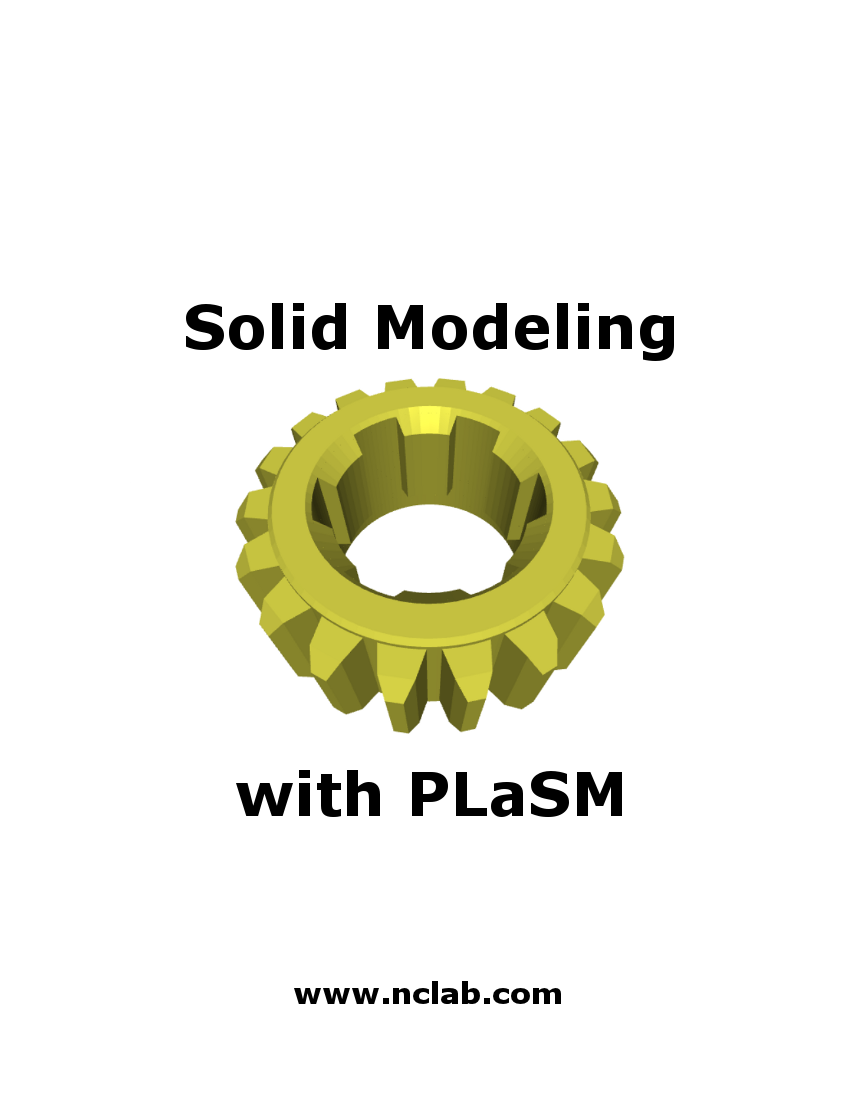
\includegraphics[width=\paperwidth,height=\paperheight]{img/plasm-frontpage.png}
%\includegraphics[width=\paperwidth,height=\paperheight]{img/background.jpg}
\vfill
}}}

\begin{document}

% INPUTTING BACKGROUND IMAGE
\AddToShipoutPicture{\BackgroundPic}
\vbox{}
\pagestyle{empty}
\newpage
\textwidth=15.5cm
\ClearShipoutPicture
\newpage

%%%%%%%%%%%%%%%%%%%%%%%%%%%%%%%%%%%%%%%%%%%%%%%%%%%%%%%%%%%%%%%%%%%%%%%%%

\section*{}
\small
\subsection*{About NCLab}
Networked Computing Laboratory (NCLab) is a popular Internet-based framework for 
programming, mathematics, computer modeling, 
and scientific computing. It serves students, instructors, researchers, and the general 
public. NCLab can be used free of charge for personal non-commercial purposes such as 
private hobby or self-education, as well as for individual non-funded academic research.
All other use is subject to {\bf purchasing a license} for a symbolic fee. The fees are as low as 
\$1 per user per month for educational use, and they are used to support the development 
and operational expenses. NCLab is a product of FEMhub Inc. The name "NCLab" is 
registered with the U.S. Patent and Trademark Office (USPTO) under Trademark No. 85420518.

\subsection*{Terms of Use and Pricing}
More details on purchasing a license and using NCLab are provided in the online documents 
{\bf Pricing} and {\bf Terms of Use} that are accessible from NCLab's home page 
{\tt http://nclab.com}.

\subsection*{Contact Information}
General inquiries: {\tt info@femhub.com}\\
Sales: {\tt sales@femhub.com}\\
NCLab support: {\tt support@nclab.com}\\
Agros \& Hermes support: {\tt support@femhub.com}\\
Web page: {\tt http://femhub.com}\\
{Physical address}\\
FEMhub Inc.\\
5490 Twin Creeks Dr.\\
Reno, NV 89523

\subsection*{About This Publication}
This publication can be copied and distributed without any restrictions
as long as reference to NCLab and FEMhub Inc. is preserved.

\subsection*{Acknowledgement}
This publication features PLaSM, an open source Programming Language for 
Solid Modeling, developed by Alberto Paoluzzi, Giorgio Scorzelli, and their 
students and collaborators at the University of Rome in Italy. Some examples 
shown here come from the original PLaSM repository. Alberto's 
and Giorgio's help and support are gratefully acknowledged. 

\normalsize

\newpage
%{\ }
\setcounter{tocdepth}{2}
\tableofcontents
%\pagestyle{plain}

\newpage

\pagestyle{plain}
\setcounter{page}{1}

%%%%%%%%%%%%%%%%%%%%%%%%%%%%%%%%%%%%%%%%%%%%%%%%%%%%%%%%%%%%%%%%%%%%%%%%%

\section{What is PLaSM?}

PLaSM ({\em Programming Language for Solid Modeling}) is a powerful design language
that enables geometrical modeling of 3D objects via simple commands.
The language was developed by the CAD Group at the Universities of Roma 
"La Sapienza" and "Roma Tre" in Italy. It is based on FL, an advanced 
language for functional programming developed by the Functional 
Programming Group at the IBM Research Center.\\

\noindent
PLaSM makes it possible to define a wide range of simple 3D objects, transform 
them, create intersections and unions via simple logical operations, and much 
more. This tutorial will guide you in small steps and using many examples
through PLaSM's usage. Soon, you will be able to create advanced 
3D geometries such as the one shown in Fig. \ref{fig:pisa}.

\begin{figure}[!ht]
\begin{center}

\includegraphics[width=0.8\textwidth]{img/temple0.png}
\end{center}
\vspace{-2mm}
\caption{Sample PLaSM model (available as Displayed Project "Temple").}
\label{fig:pisa}
\end{figure}

\section{Getting Started}

In order to make the most of this tutorial, we invite the 
reader to create an account in NCLab and log in. More instructions 
on how to do this are given at the beginning of the introductory 
tutorial "Meet Your New Graphing Calculator" that is available in 
PDF via a link on NCLab home page {\tt http://nclab.com}. \\

\noindent
{\bf NOTE}: Your web browser needs to support WebGL, otherwise you will not be able to 
work with PLaSM properly. For this reason, a WebGL test button is provided 
on NCLab's front page.\\

\noindent
After logging in, you will see a desktop with several icons on it,
as shown in Fig. \ref{fig:desktop}. 

\begin{figure}[!ht]
\begin{center}
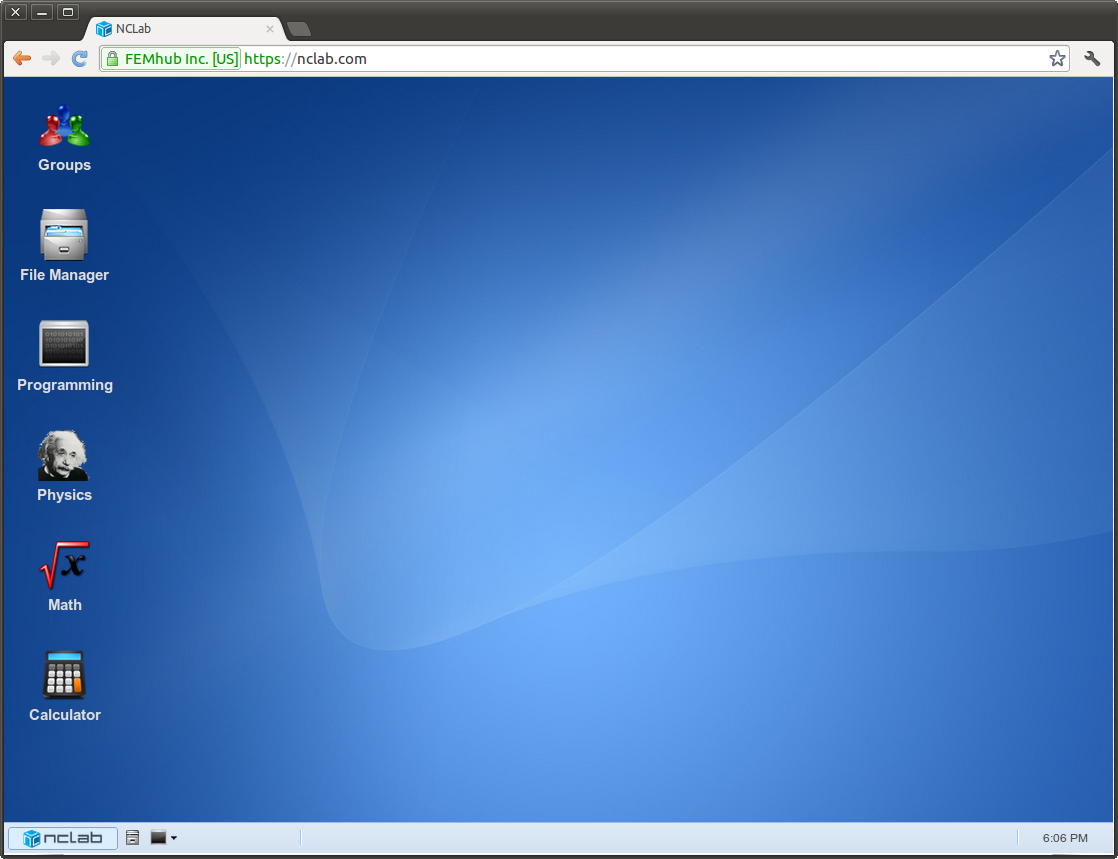
\includegraphics[width=\textwidth]{img/desktop.png}
\end{center}
%\vspace{-2mm}
\caption{NCLab desktop after login.}
\label{fig:desktop}
\end{figure}

\subsection{Cloning Displayed Projects}

All examples that we are going to work with in the following are also available 
as Displayed Projects. This means that you can clone them by launching the File
Manager, going to the {\em Project} menu, and clicking on {\em Clone}. This will launch 
a window with many displayed projects from various areas of programming,
math and computing. Look for projects whose names start with "PLaSM - Tutorial".
After you locate a project that you would like to clone, click on it,
and then click on the button {\em Clone} at the bottom of the window. This will
create exact copy of that project in your account, and you can open it 
by clicking on it in the File Manager. You can change the project in any way 
you like, the changes will not affect the original Displayed Project. 


\subsection{Launching a new Python project}

Alternatively, you can type the examples by yourself, which is the 
recommended way. Our introductory examples have no more than 
a couple of lines anyway. So, in the File Manager's {\em Project} menu 
choose {\em New} $\rightarrow$ {\em Python}. This will launch an 
empty Python project, as shown in Fig. \ref{fig:python}.


\begin{figure}[!ht]
\begin{center}
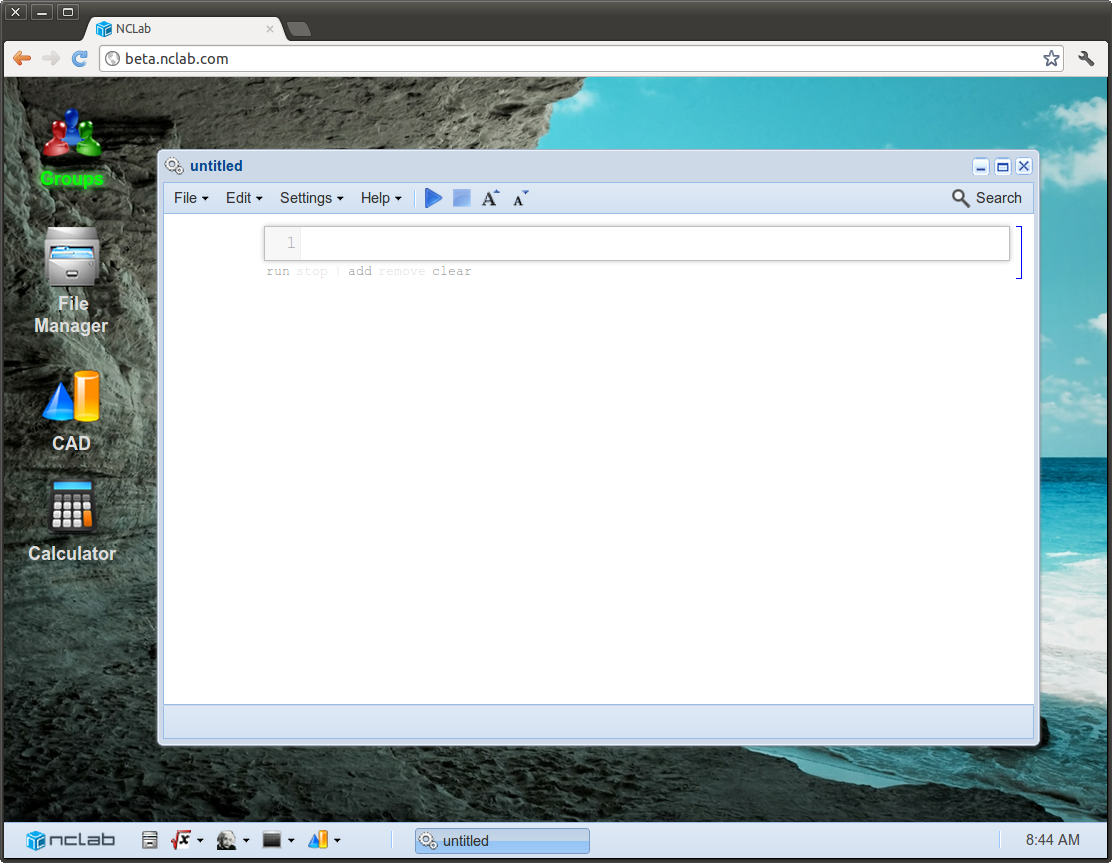
\includegraphics[width=\textwidth]{img/python.png}
\end{center}
%\vspace{-2mm}
\caption{Launching a new Python project.}
\label{fig:python}
\end{figure}
\noindent



\subsection{Creating a unit cube}

In the input cell, enter the code:

\begin{verbatim}
from pyplasm import *
cube = CUBOID([1, 1, 1])
lab.view(cube, [0.4, 0.9, 0.6])
\end{verbatim}
Then click on the link "run" under the input cell. This will send a request 
to the cloud. The answer should come back instantly, and a new WebGL widget 
with a unit cube in it should appear, as shown in Fig. \ref{fig:cube}. 
Congratulations, you just created your first PLaSM model!

\begin{figure}[!ht]
\begin{center}
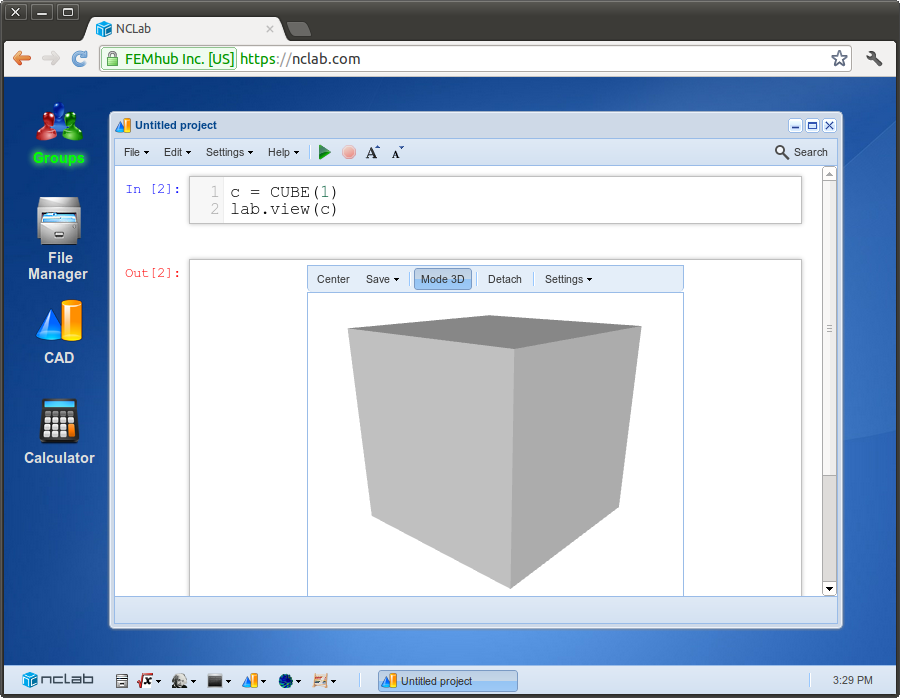
\includegraphics[width=\textwidth]{img/cube.png}
\end{center}
%\vspace{-2mm}
\caption{WebGL widget containing a unit cube.}
\label{fig:cube}
\end{figure}

\subsection{Mouse controls}

Now click into the window and move the mouse while holding the left
button pressed. The cube should freely rotate in 3D. Holding the middle
button (or the mouse wheel) pressed and moving the mouse will move the 
object to any direction. Zooming can be done with the mouse wheel or
with the right-hand mouse button.

\section{Creating Simple Objects}

Before we move on, let us briefly explain the above code.
The first line, 

\begin{verbatim}
from pyplasm import *
\end{verbatim}
imports the PLaSM library into NCLab. This is similar to how we imported
the Sympy, Numpy and Scipy libraries in the introductory course "Meet Your 
New Graphing Calculator". The second line,

\begin{verbatim}
cube = CUBOID([1, 1, 1])
\end{verbatim}
defines a 3D unit cube. The CUBOID command will be explained in more detail below.
The last line,

\begin{verbatim}
lab.view(cube, [0.4, 0.9, 0.6])
\end{verbatim}
tells NCLab to display the cube in a WebGL widget. 

\subsection{Using colors}

The triplet {\tt [0.4, 0.9, 0.6]} in the {\tt lab.view()} command
represents the RGB components defining a color. The numbers need to be between 
0.0 and 1.0. You can experiment with colors, keeping a few simple rules in mind:

\begin{itemize}
\item With just the first value being non-zero, such as in {\tt [0.5, 0, 0]},
      you get {\bf red} color. The closer the value is to 1.0, the lighter the color
      will be.
\item With just the second value being non-zero, such as in {\tt [0, 0.5, 0]},
      you obtain {\bf green} color. The closer the  value is to 1.0, the lighter the color
      will be.
\item With just the third value being non-zero, such as in {\tt [0, 0, 0.5]},
      you will have {\bf blue} color. The closer the  value is to 1.0, the lighter the color
      will be.
\item Using three identical values will result into a shade of grey. {\tt [0, 0, 0]}
      means black, {\tt [1.0, 1.0, 1.0]} means white.
\item Varying all three numbers, you can get any color that you want. It is not 
      easy to translate a color, such as "purple", "cyan" or "orange" into the RGB
      values. But there are many web pages that will do it for you, such as for
      example http://kb.iu.edu/data/aetf.html. {\bf Note}: Usually,
      the RGB values on these web pages are given as integers between 0 and 255. To use them in NCLab,
      just divide all three of them by 255.
\end{itemize}

 
\subsection{Brick, cube, rectangle, and square -- command CUBOID}

Why is the command called 
CUBOID and not CUBE? The answer is -- because the command covers more 
than cubes. With three parameters {\tt [a, b, c]} it will render 
a 3D brick with edge lengths {\tt a}, {\tt b} and {\tt c}. Let us change the 
above code to  

\begin{verbatim}
from pyplasm import *
cube = CUBOID([3, 2, 1])
lab.view(cube, [0.4, 0.9, 0.6])
\end{verbatim}
and press the "run" link under the input cell again. The result is 
displayed in Fig. \ref{fig:cuboid-1}.


\begin{figure}[!ht]
\begin{center}
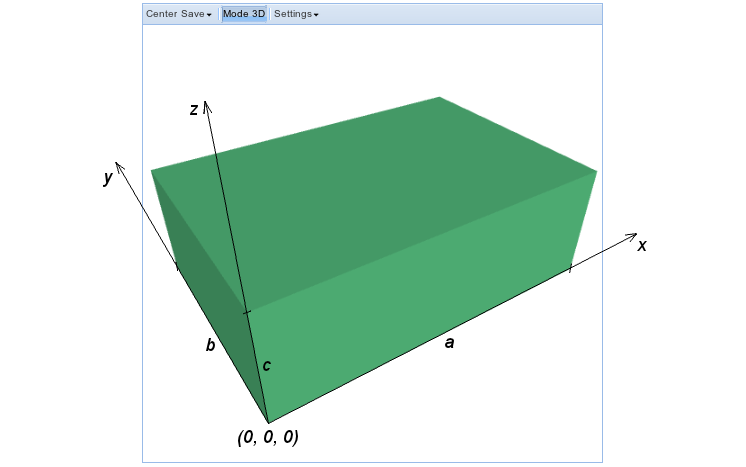
\includegraphics[width=0.8\textwidth]{img/cuboid-1.png}
\end{center}
\vspace{-2mm}
\caption{CUBOID([3, 2, 1]) generates a brick with edge lenghts 3, 2 and 1.}
\label{fig:cuboid-1}
\end{figure}
\noindent
With two parameters {\tt [a, b]} the CUBOID command will render a 2D rectangle 
(2D brick if you like) with edge lengths {\tt a} and {\tt b}, as shown in 
Fig. \ref{fig:cuboid-2}

\newpage

\begin{figure}[!ht]
\begin{center}
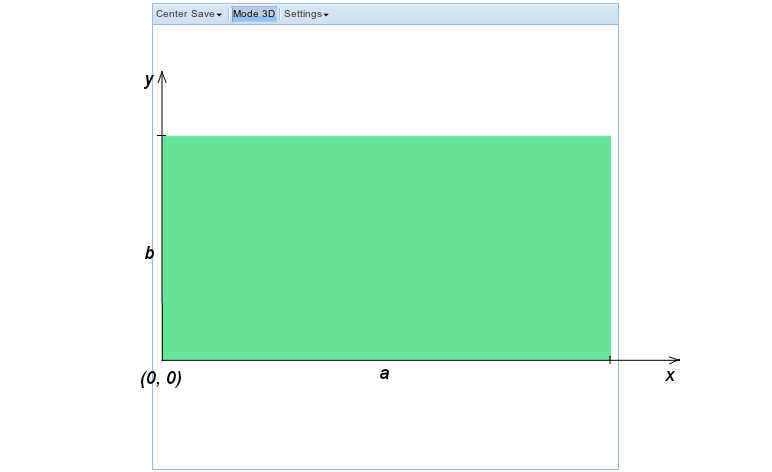
\includegraphics[width=0.82\textwidth]{img/cuboid-2.png}
\end{center}
\vspace{-2mm}
\caption{CUBOID([2, 1]) generates a rectangle with edge lenghts 2 and 1.}
\label{fig:cuboid-2}
%\vspace{-1cm}
\end{figure}


\subsection{Unit tetrahedron and triangle -- command SIMPLEX}

A unit tetrahedron (unit 3D simplex) can be created using the code
\begin{verbatim}
from pyplasm import *
tet = SIMPLEX(3)
lab.view(tet, [0.4, 0.9, 0.6])
\end{verbatim}
The output of the above code is shown in Fig. \ref{fig:simplex-1}.

\newpage

\begin{figure}[!ht]
\begin{center}
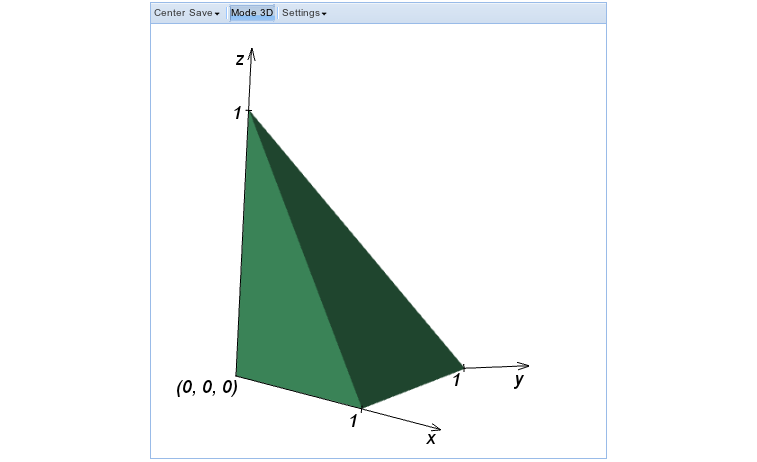
\includegraphics[width=0.82\textwidth]{img/simplex-1.png}
\end{center}
\vspace{-2mm}
\caption{SIMPLEX(3) generates a unit 3D simplex (unit tetrahedron).}
\label{fig:simplex-1}
\end{figure}
\noindent
Note -- in the next paragraph we will show how to create a general 
tetrahedron using the 
A unit triangle (unit 2D simplex) can be created using the code
\begin{verbatim}
from pyplasm import *
tria = SIMPLEX(2)
lab.view(tria, [0.4, 0.9, 0.6])
\end{verbatim}
The output of the above code is shown in Fig. \ref{fig:simplex-2}.
\newpage

\begin{figure}[!ht]
\begin{center}
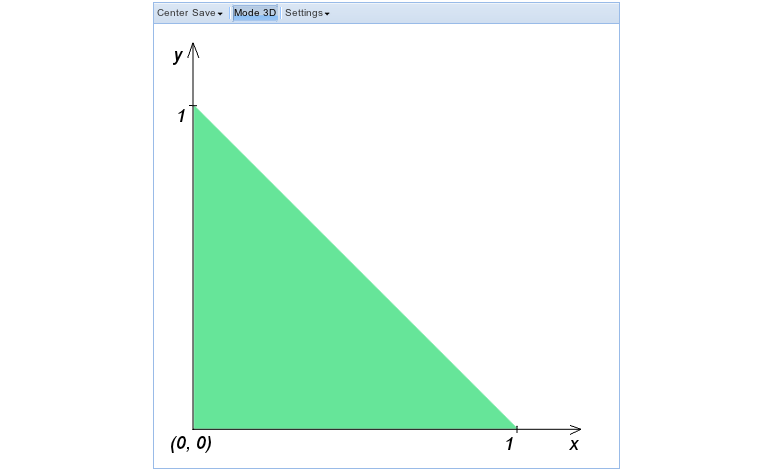
\includegraphics[width=0.82\textwidth]{img/simplex-2.png}
\end{center}
\vspace{-2mm}
\caption{SIMPLEX(2) generates a unit 2D simplex (triangle).}
\label{fig:simplex-2}
\vspace{-1cm}
\end{figure}

\subsection{General tetrahedron and triangle}

The command CONVEXHULL is a powerful tool to define convex 3D and 2D objects using 
their corner points. In particular it can be used to create general tetrahedra and 
triangles. The command takes a list of points as an argument. For example, the code

\begin{verbatim}
from pyplasm import *
points = [[-1, 0, 0], [1, 0, 0], [0, 4, 1], [0, 1, 5]]
tetra = CONVEXHULL(points)
lab.view(tetra, [0.4, 0.9, 0.6])
\end{verbatim}
creates a tetrahedron with vertices $[-1, 0, 0]$, $[1, 0, 0]$, $[0, 4, 1]$ and $[0, 1, 5]$.
The code

\begin{verbatim}
from pyplasm import *
points = [[1, 1], [4, 2], [2, 4]]
tria = CONVEXHULL(points)
lab.view(tria, [0.4, 0.9, 0.6])
\end{verbatim}
generates a triangle with the vertices $[1, 1]$, $[4, 2]$ and $[2, 4]$. In this way 
the reader can define any convex polytop in 3D or polygon in 2D -- just using more 
points!

\subsection{Command CONVEXHULL}

Let us demonstrate the true power of PLaSM by writing a simple program that generates 
a polygon with $N$ equally-long edges that is inscribed into a circle of radius $R$.
For this example, you need to know elementary commands of the Python programming 
language. If you have never programmed in Python, do not worry and skip to the next 
example. Eventually, read the tutorial on Python Programming that is also provided
in NCLab.

\begin{verbatim}
from pyplasm import *
from numpy import sin, cos, pi
N = 15
R = 5
points = []
for i in range(N):
    angle = i * 2. * pi / N
    points.append([R * cos(angle), R * sin(angle)])
polygon = CONVEXHULL(points)
lab.view(polygon, [0.4, 0.9, 0.6])
\end{verbatim}
The output of the above code is shown in Fig. \ref{fig:convexhull-1}.

\begin{figure}[!ht]
\begin{center}
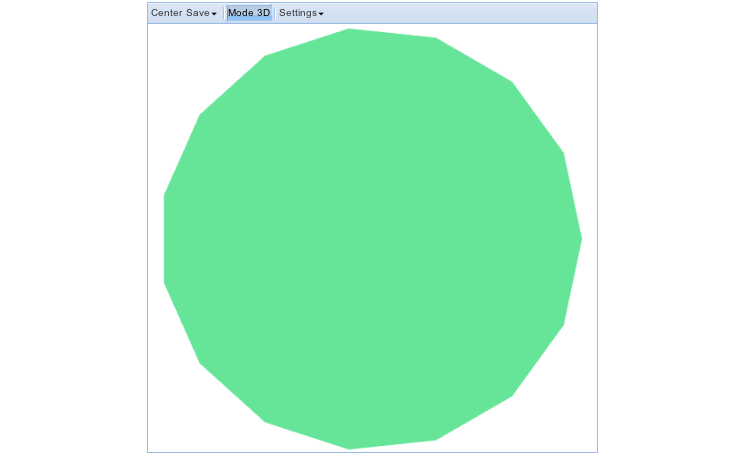
\includegraphics[width=0.82\textwidth]{img/convexhull-1.png}
\end{center}
\vspace{-2mm}
\caption{Polygon with 15 equally long edges inscribed into a circle.}
\label{fig:convexhull-1}
%\vspace{-1cm}
\end{figure}

\subsection{Circle via convex hull}

When the parameter $N$ is increased to 128 or 256 in the last program, 
one obtains a {\bf circle}. This is in fact the way circles are handled in PLaSM.
 

\subsection{Cone via convex hull}

The CONVEXHULL command has amazing power. Let us tweak the code
from the previous paragraph a bit to construct a cone of radius
$R$ and height $H$. All we need to do is to add a zero third coordinate 
to the points generated in the previous program, and add one more 
point -- the tip of the cone. The CONVEXHULL command will take care 
of the rest:

{\small
\begin{verbatim}
from pyplasm import *
from numpy import sin, cos, pi
R = 5
H = 10
points = []
subdiv = 128
for i in range(N):
    angle = i * 2. * pi / subdiv
    points.append([R * cos(angle), R * sin(angle), 0])
points.append([0, 0, H])
cone = CONVEXHULL(points)
lab.view(cone, [0.4, 0.9, 0.6])
\end{verbatim}
}
\noindent
The output of the above code is shown in Fig. \ref{fig:convexhull-2}.

\begin{figure}[!ht]
\begin{center}
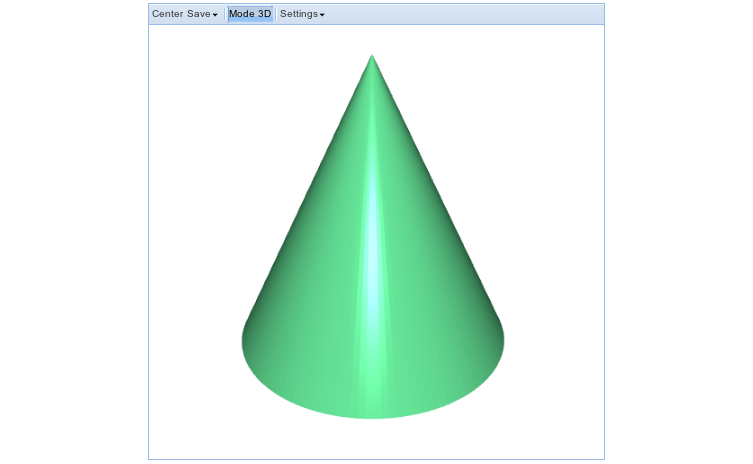
\includegraphics[width=0.82\textwidth]{img/convexhull-2.png}
\end{center}
\vspace{-2mm}
\caption{Cone of radius $R$ and height $H$.}
\label{fig:convexhull-2}
\vspace{-1cm}
\end{figure}
\newpage
The subdivision {\tt subdic = 128} is how many
faces are used to approximate the round surface. You may use less, 
for example 64 or even 32, which will make the rendering faster, but
the surface will be less smooth. On the other hand, with more than 
128 subdivisions the surface will be even more smooth-looking, but 
the rendering will take longer.

\subsection{Command CYLINDER}

We have no doubt that the reader would be able to construct 
a cylinder of radius $R$ and height $H$ via convex hull. 
In fact, you may try it as a simple exercise, starting from 
the program for the cone. But, PLaSM has a specific command
CYLINDER for that:

\begin{verbatim}
from pyplasm import *
R = 0.25
H = 1.0
cyl = CYLINDER ([R, H])(128)
lab.view(cyl, [0.4, 0.9, 0.6])
\end{verbatim}
The cylinder's axis is in the $z$-direction, and the midpoint of
its base circle is the origin $[0, 0, 0]$. 
The output of the above code is shown in Fig. \ref{fig:cyl-1}.

\begin{figure}[!ht]
\begin{center}
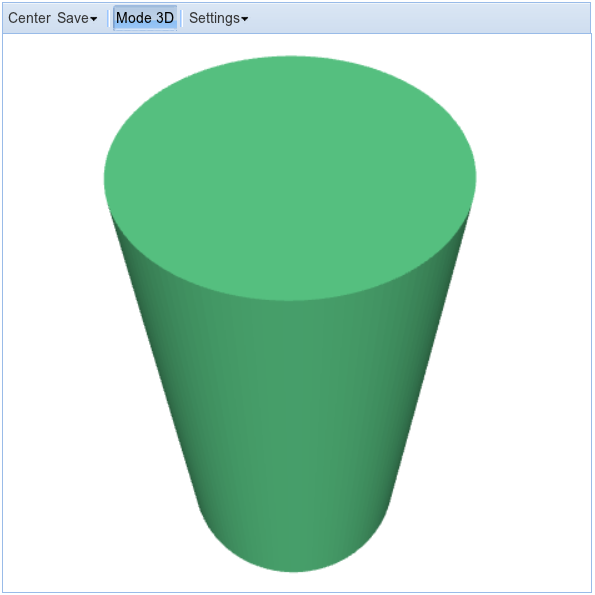
\includegraphics[width=0.5\textwidth]{img/cyl-1.png}
\end{center}
\vspace{-2mm}
\caption{Cylinder of radius $R$ and height $H$.}
\label{fig:cyl-1}
%\vspace{-1cm}
\end{figure}

\subsection{Command TUBE}

A hollow tube of inner radius $r$, outer radius $R$ and height
$H$ is rendered using the TUBE command. It is used as follows:
\begin{verbatim}
from pyplasm import *
r = 0.9
R = 1.0
H = 3.0
tube = TUBE([r, R, H])(128)
lab.view(tube, [0.4, 0.9, 0.6])
\end{verbatim}
The tube's axis is in the $z$-direction, and the midpoint of
its base circle is the origin $[0, 0, 0]$. Again, the parameter
128 is the number of linear faces that approximate the 
curved surfaces. The output of the above code is shown in Fig. \ref{fig:tube-1}.

\begin{figure}[!ht]
\begin{center}
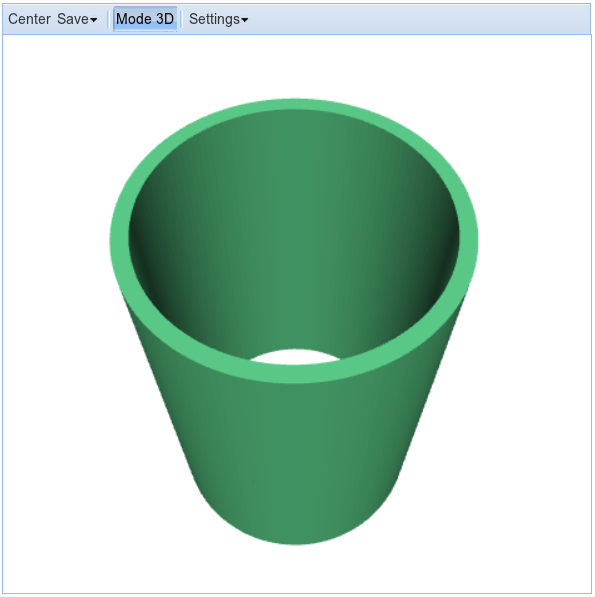
\includegraphics[width=0.5\textwidth]{img/tube-1.png}
\end{center}
\vspace{-2mm}
\caption{Tube of inner radius $r$, outer radius $R$ and height $H$.}
\label{fig:tube-1}
%\vspace{-1cm}
\end{figure}

\subsection{Command SPHERE}

A sphere of radius $R$ is rendered using the command SPHERE.
For example, the code

\begin{verbatim}
from pyplasm import *
R = 1.0
s = SPHERE(3.0)([64, 64])
lab.view(s, [0.4, 0.9, 0.6])
\end{verbatim}
will render a unit sphere whose origin is at $[0, 0, 0]$. 
The parameter {\tt [64, 64]} stands for 
subdivision in both tangential directions. We need to be a bit 
careful with increasing this number, since doubling it to 
{\tt [128, 128]} would increase 
the number of linear faces approximation the sphere {\bf four times}.
The output of the above code is shown in Fig. \ref{fig:sphere-1}.

\begin{figure}[!ht]
\begin{center}
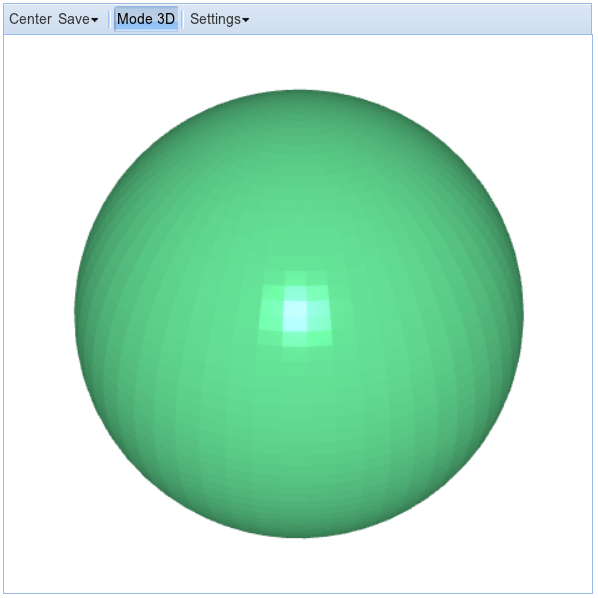
\includegraphics[width=0.5\textwidth]{img/sphere-1.png}
\end{center}
\vspace{-2mm}
\caption{Sphere of radius $R$ and origin $[0, 0, 0]$.}
\label{fig:sphere-1}
%\vspace{-1cm}
\end{figure}


\subsection{Command TORUS}

The TORUS command takes an inner radius $r$ and outer radius 
$R$ as parameters. It is used as follows:
\begin{verbatim}
from pyplasm import *
r = 3.0
R = 5.0
tor = TORUS([r, R])([64, 64])
lab.view(tor, [0.4, 0.9, 0.6])
\end{verbatim}
The center of the torus is at the origin $[0, 0, 0]$ and its axis
is the $z$-axis. This is illustrated in Fig. \ref{fig:torus-1}.

\begin{figure}[!ht]
\begin{center}
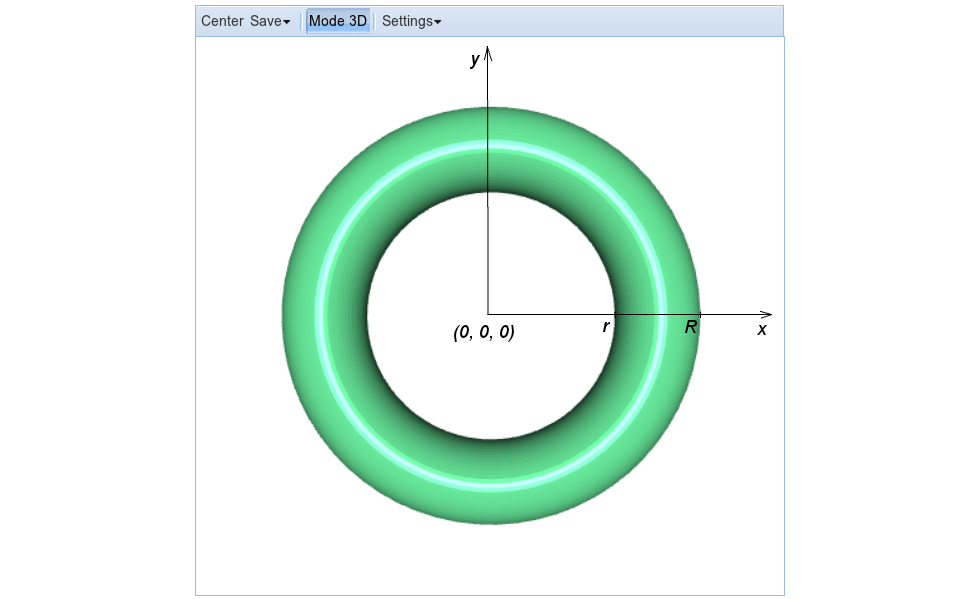
\includegraphics[width=0.82\textwidth]{img/torus-1.png}
\end{center}
\vspace{-2mm}
\caption{Torus of inner radius $r$, outer radius $R$ and center at the origin $[0, 0, 0]$.}
\label{fig:torus-1}
%\vspace{-1cm}
\end{figure}



\subsection{Exercises}

Solutions to all exercises from this section are available in the Solution Manual, and 
they can be also cloned in NCLab through Project $\rightarrow$ Clone in the 
File Manager's menu.\\

\noindent
\underline{\em Exercise A1: Blue brick}

Create a $3 \times 4 \times 5$ brick in a light
blue color, as shown in Fig. \ref{fig:a1}.

\newpage

\begin{figure}[!ht]
\begin{center}
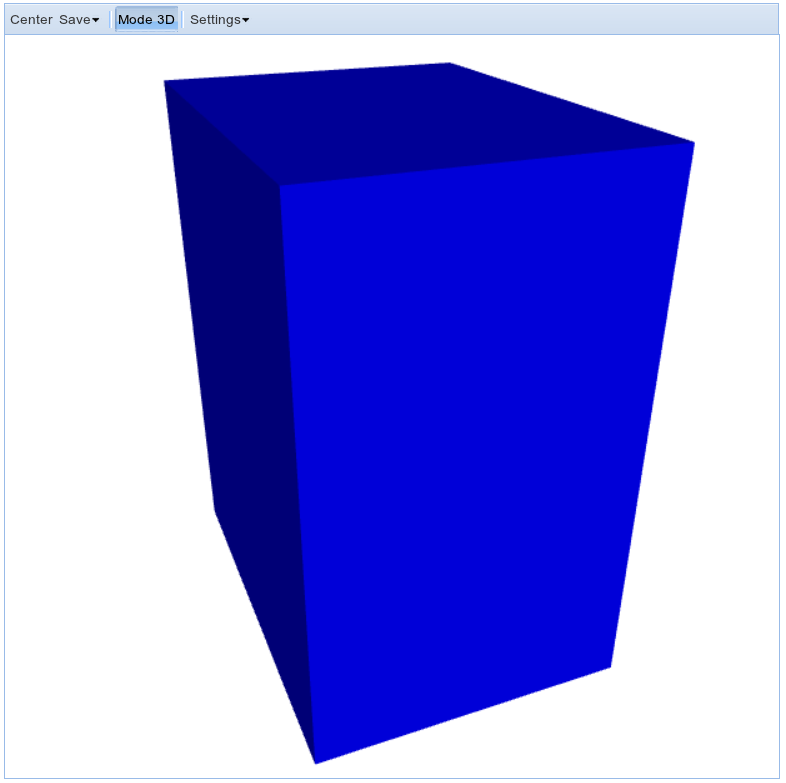
\includegraphics[width=0.5\textwidth]{img/a1-blue-brick.png}
\end{center}
\vspace{-2mm}
\caption{Illustration for Exercise A1.}
\label{fig:a1}
%\vspace{-1cm}
\end{figure}


\noindent
\underline{\em Exercise A2: Red rectangle}

Create a $3 \times 1$ rectangle in a light
red color, as shown in Fig. \ref{fig:a2}.

\begin{figure}[!ht]
\begin{center}

\includegraphics[width=0.5\textwidth]{img/a2-red-rectangle.png}
\end{center}
\vspace{-2mm}
\caption{Illustration for Exercise A2.}
\label{fig:a2}
\vspace{-1cm}
\end{figure}
\newpage
\noindent
\underline{\em Exercise A3: Orange Octahedron}

Create an orange octahedron with vertices 
$[0, -1, 1]$, $[0, 1, 1]$, $[0, -1, -1]$, $[0, 1, -1]$, $[2, 0, 0]$, and $[-2, 0, 0]$, 
as shown in Fig. \ref{fig:a3}.

\begin{figure}[!ht]
\begin{center}
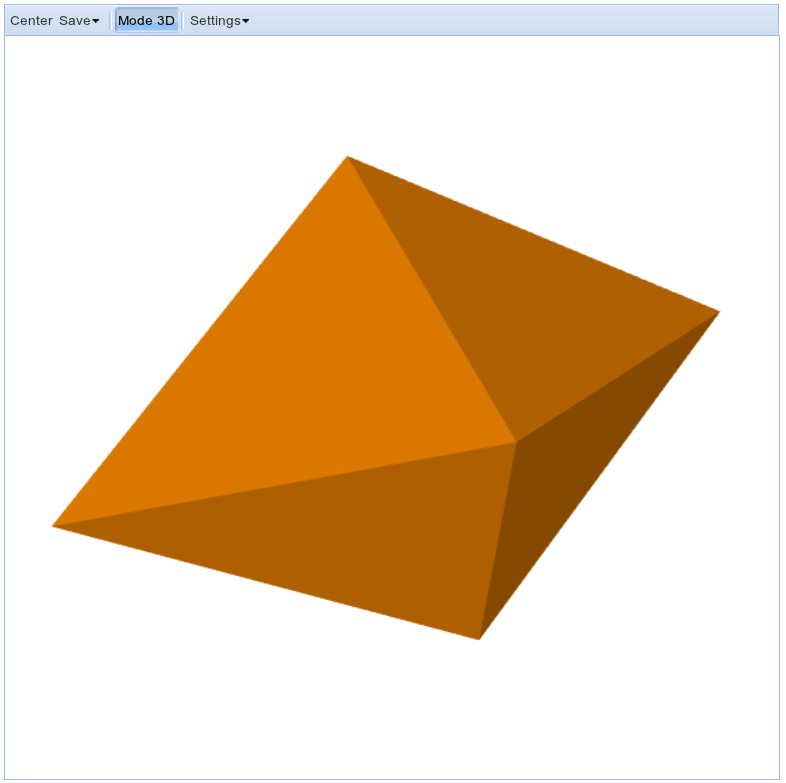
\includegraphics[width=0.5\textwidth]{img/a3-orange-octahedron.png}
\end{center}
\vspace{-2mm}
\caption{Illustration for Exercise A3.}
\label{fig:a3}
%\vspace{-1cm}
\end{figure}

\noindent
\underline{\em Exercise A4: Pink Pentagon}

Create a pink pentagon with equally-long edges that is inscribed 
in a circle with diameter $R$, as shown in Fig. \ref{fig:a4}.

\newpage

\begin{figure}[!ht]
\begin{center}
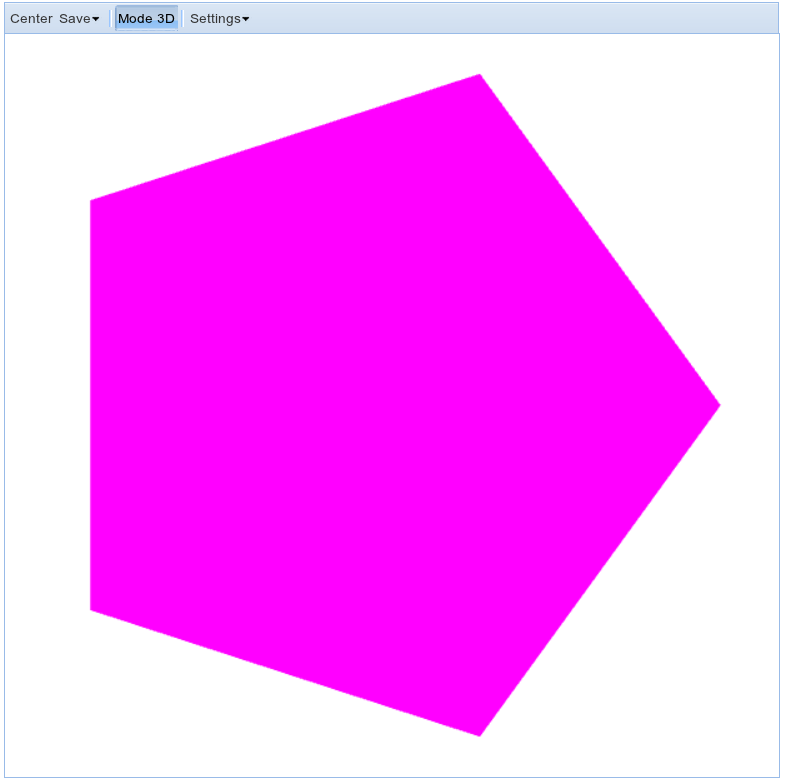
\includegraphics[width=0.5\textwidth]{img/a4-pink-pentagon.png}
\end{center}
\vspace{-4mm}
\caption{Illustration for Exercise A4.}
\label{fig:a4}
\vspace{-4mm}
\end{figure}

\noindent
\underline{\em Exercise A5: Cyan Cone}

Create a cyan cone of radius $R$ and height $H$ that stands on its tip
(the tip is at $[0, 0, 0]$ and the axis of the cone coincides with the 
$z$-axis), as shown in Fig. \ref{fig:a5}.

\begin{figure}[!ht]
\begin{center}
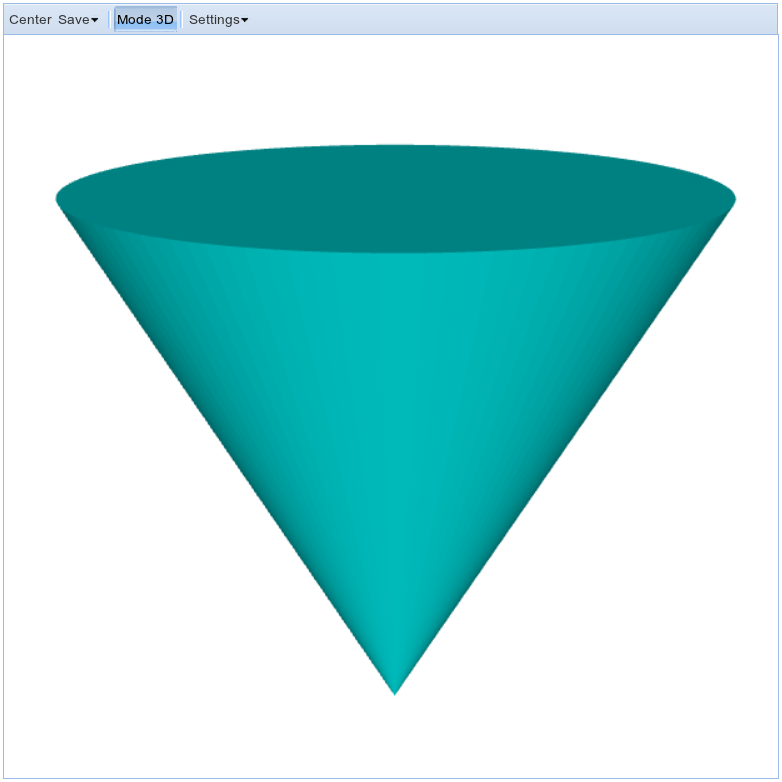
\includegraphics[width=0.5\textwidth]{img/a5-cyan-cone.png}
\end{center}
\vspace{-4mm}
\caption{Illustration for Exercise A5.}
\label{fig:a5}
\vspace{-1cm}
\end{figure}

\newpage
\noindent
\underline{\em Exercise A6: Carmine Cylinder}

Create a carmine cylinder of radius $R$ and height $H$, 
as shown in Fig. \ref{fig:a6}.

\begin{figure}[!ht]
\begin{center}
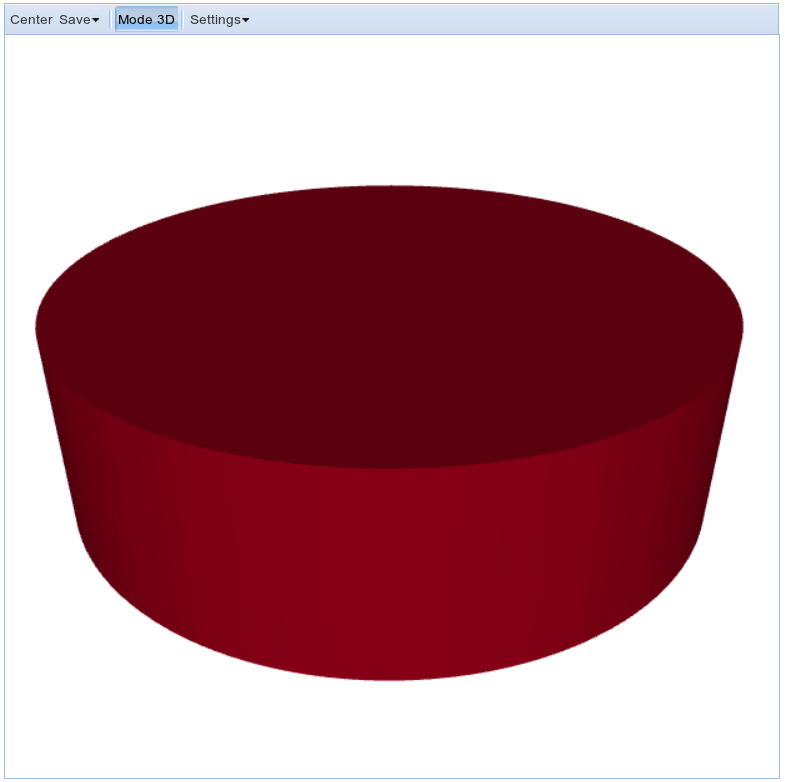
\includegraphics[width=0.5\textwidth]{img/a6-carmine-cylinder.png}
\end{center}
\vspace{-2mm}
\caption{Illustration for Exercise A6.}
\label{fig:a6}
%\vspace{-1cm}
\end{figure}

\noindent
\underline{\em Exercise A7: Topaz Tube}

Create a topaz tube of inner radius $R_{in}$, outer radius $R_{out}$
and height $H$, as shown in Fig. \ref{fig:a7}.

\newpage

\begin{figure}[!ht]
\begin{center}
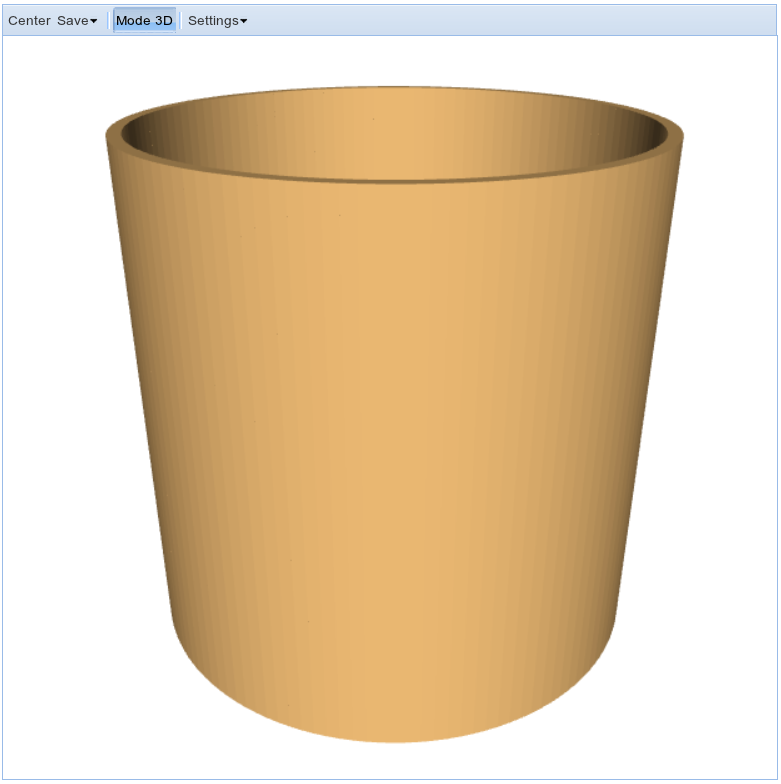
\includegraphics[width=0.5\textwidth]{img/a7-topaz-tube.png}
\end{center}
\vspace{-2mm}
\caption{Illustration for Exercise A7.}
\label{fig:a7}
%\vspace{-1cm}
\end{figure}


\noindent
\underline{\em Exercise A8: Sand Sphere}

Create a sand sphere of radius $R$ and center at the origin $[0, 0, 0]$. 
Use $[64, 64]$ for the piecewise-linear approximation of the curved surface, 
as shown in Fig. \ref{fig:a8}.

\newpage

\begin{figure}[!ht]
\begin{center}
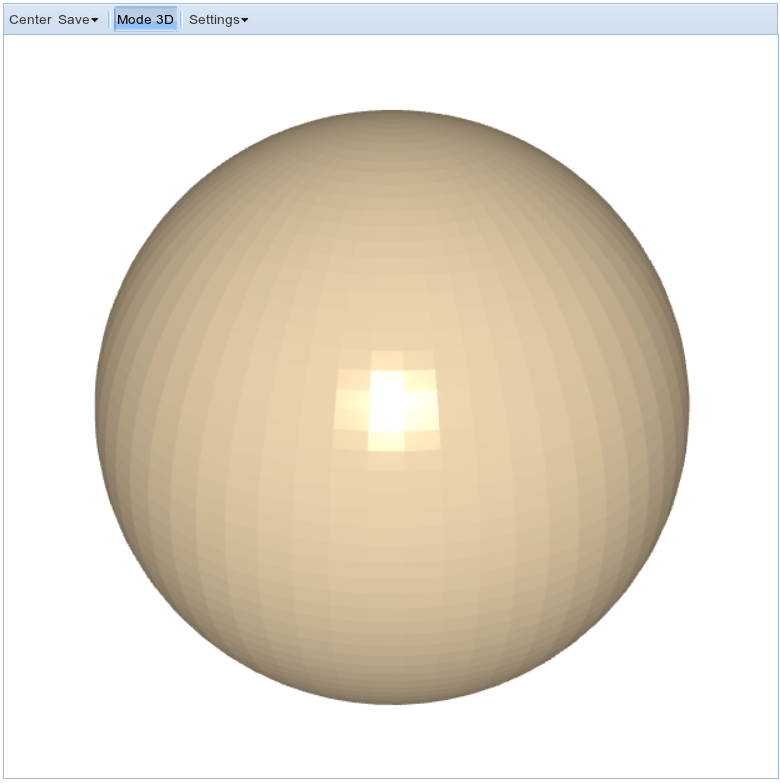
\includegraphics[width=0.5\textwidth]{img/a8-sand-sphere.png}
\end{center}
\vspace{-2mm}
\caption{Illustration for Exercise A8.}
\label{fig:a8}
%\vspace{-1cm}
\end{figure}

\noindent
\underline{\em Exercise A9: Turquoise Torus}

Create a turquoise torus of inner radius $R_{in}$ and outer radius $R_{out}$, whose center 
is at the origin $[0, 0, 0]$. Use $[64, 64]$ for the piecewise-linear approximation 
of the curved surface, as shown in Fig. \ref{fig:a9}.

\newpage

\begin{figure}[!ht]
\begin{center}
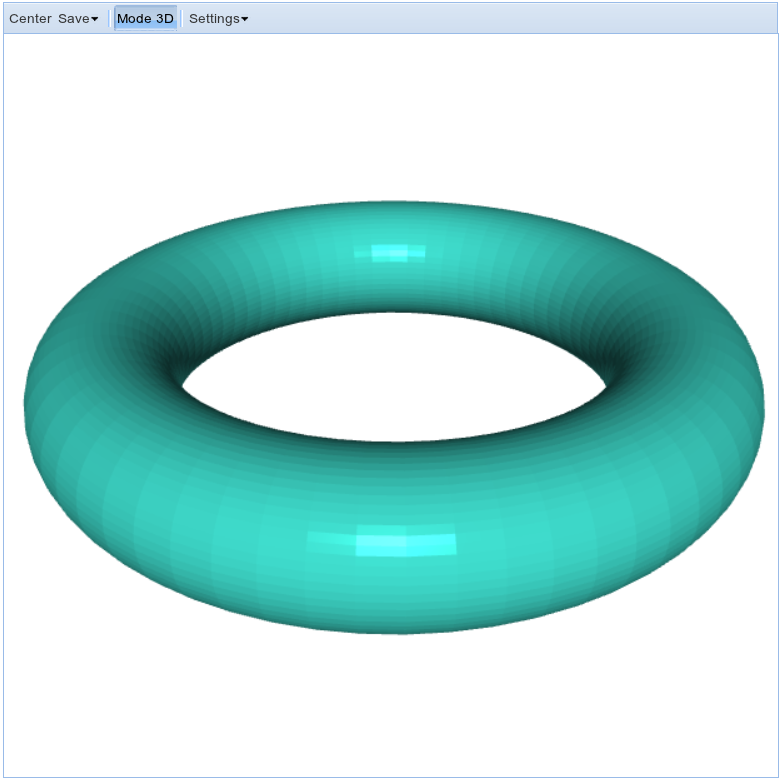
\includegraphics[width=0.5\textwidth]{img/a9-turquoise-torus.png}
\end{center}
\vspace{-2mm}
\caption{Illustration for Exercise A9.}
\label{fig:a9}
\vspace{-1cm}
\end{figure}

\section{Transformations}

So far we have learned how to create a variety of simple 2D and 3D objects. 
The next step is to learn how to scale, rotate, and translate them. PLaSM
provides simple commands for that. Let us begin with scaling.

\subsection{Command SCALE}

The SCALE command takes three arguments: A list of axial directions in which 
the object will be scaled (as integers), list of scaling factors for these 
directions, and the object to be scaled. For example, let us create a cylinder 
{\tt cyl} of radius 1.0 and height 0.3:

\begin{verbatim}
from pyplasm import *
cyl = CYLINDER([1.0, 0.3])(128)
\end{verbatim}
We know from before that the axis of this cylinder coincides with the $z$-axis 
and that the center of its bottom face is at $[0, 0, 0]$. The output is shown in Fig. \ref{fig:scale-0}.

\newpage

\begin{figure}[!ht]
\begin{center}
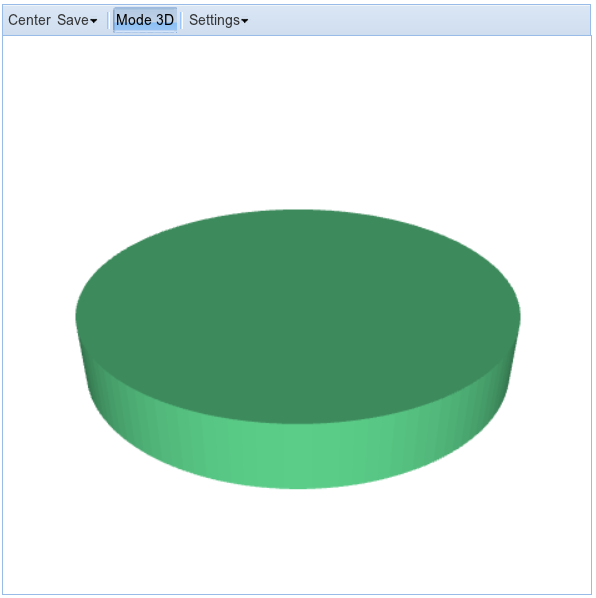
\includegraphics[width=0.5\textwidth]{img/scale-0.png}
\end{center}
\vspace{-2mm}
\caption{Cylinder of radius 1.0 and height 0.3.}
\label{fig:scale-0}
%\vspace{-1cm}
\end{figure}

\noindent
\underline{\em Scaling in $x$-direction}\\

The following command will 
scale the cylinder in the $x$-direction by the factor of 2.0: 

\begin{verbatim}
cyl1 = SCALE([1])([2.0])(cyl)
lab.view(cyl1, [0.4, 0.9, 0.6])
\end{verbatim}
In fact, the $x$-coordinate of all points forming 
the object will be multiplied by 2.0. So, the axis of the resulting object will still
coincide with the $z$-axis, and the center of its bottom face will
still be at the origin $[0, 0, 0]$. Only its limits in the $x$-direction will change 
from $[-1.0, 1.0]$ to $[-2.0, 2.0]$.
The output is shown in Fig. \ref{fig:scale-1}.

\newpage

\begin{figure}[!ht]
\begin{center}
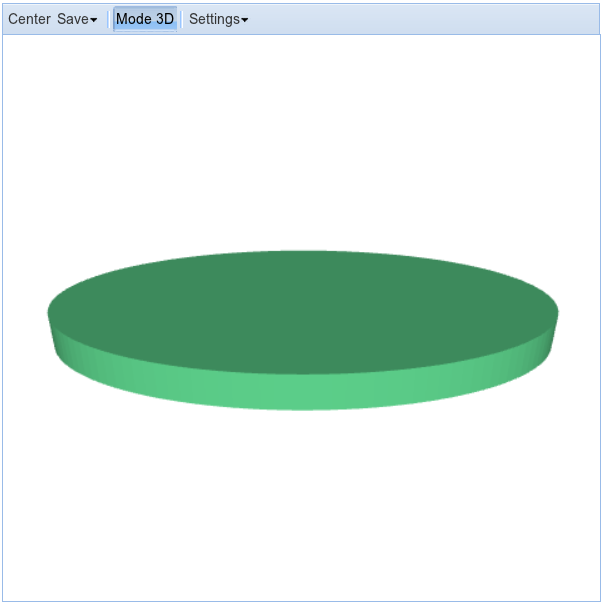
\includegraphics[width=0.5\textwidth]{img/scale-1.png}
\end{center}
\vspace{-2mm}
\caption{Cylinder scaled in the first axial direction by 2.0.}
\label{fig:scale-1}
%\vspace{-1cm}
\end{figure}

\noindent
\underline{\em Scaling in $y$-direction}\\

The following command will 
scale the cylinder in the $y$-direction by the factor of 2.0: 

\begin{verbatim}
cyl2 = SCALE([2])([2.0])(cyl)
lab.view(cyl2, [0.4, 0.9, 0.6])
\end{verbatim}
The axis of the resulting object will still
coincide with the $z$-axis, and the center of its bottom face will
still be at the origin $[0, 0, 0]$. Only its limits in the $y$-direction will change 
from $[-1.0, 1.0]$ to $[-2.0, 2.0]$.
The output is shown in Fig. \ref{fig:scale-2}.

\newpage

\begin{figure}[!ht]
\begin{center}
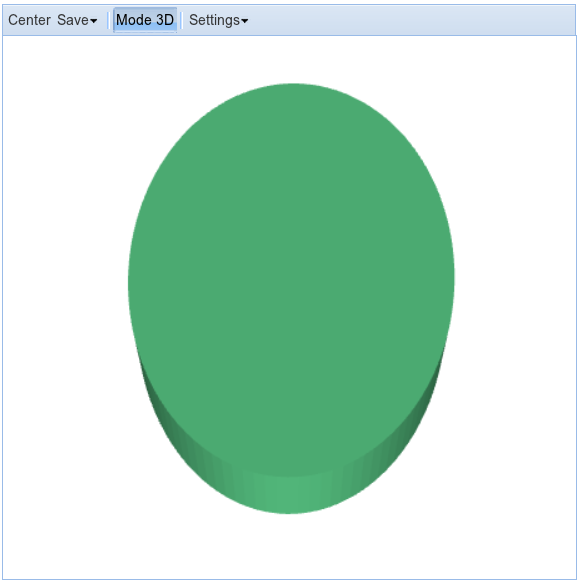
\includegraphics[width=0.5\textwidth]{img/scale-2.png}
\end{center}
\vspace{-2mm}
\caption{Cylinder scaled in the second axial direction by 2.0.}
\label{fig:scale-2}
%\vspace{-1cm}
\end{figure}

\noindent
\underline{\em Scaling in $z$-direction}\\

The following command will 
scale the cylinder in the $z$-direction by the factor of 2.0: 

\begin{verbatim}
cyl3 = SCALE([3])([2.0])(cyl)
lab.view(cyl3, [0.4, 0.9, 0.6])
\end{verbatim}
The axis of the resulting object will still
coincide with the $z$-axis, and the center of its bottom face will
still be at the origin $[0, 0, 0]$. Only its limits in the $z$-direction will change 
from $[0.0, 0.3]$ to $[0.0, 0.6]$. The output is shown in Fig. \ref{fig:scale-3}.

\newpage

\begin{figure}[!ht]
\begin{center}
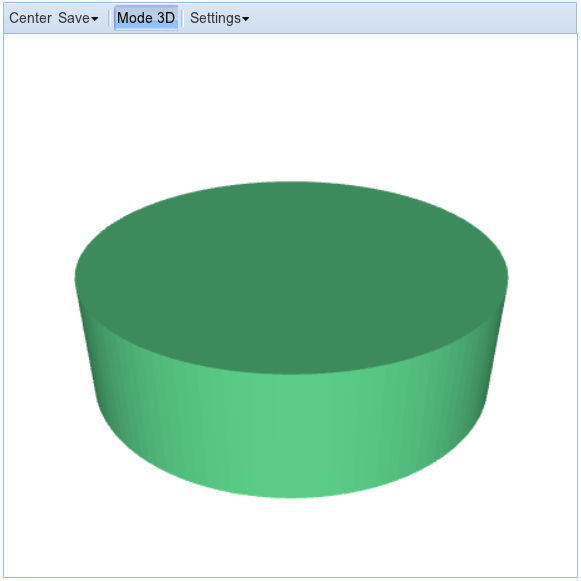
\includegraphics[width=0.5\textwidth]{img/scale-3.png}
\end{center}
\vspace{-2mm}
\caption{Cylinder scaled in the third axial direction by 2.0.}
\label{fig:scale-3}
%\vspace{-1cm}
\end{figure}

\noindent
\underline{\em Scaling in $x$ and $z$ directions simultaneously}\\

The following command will 
scale the cylinder simultaneously in the $x$- directions by 2.0 and in the $z$-direction by 4.0.
This can be viewed as scaling in the $xz$-plane:

\begin{verbatim}
cyl4 = SCALE([1, 3])([2.0, 4.0])(cyl)
lab.view(cyl4, [0.4, 0.9, 0.6])
\end{verbatim}
The axis of the resulting object will still
coincide with the $z$-axis, and the center of its bottom face will
still be at the origin $[0, 0, 0]$. Only its limits in the $x$-direction 
will change from $[-1.0, 1.0]$ to $[-2.0, 2.0]$, and the limits in the 
$z$-direction will change 
from $[0.0, 0.3]$ to $[0.0, 1.2]$. The output is shown in Fig. \ref{fig:scale-4}.

\newpage

\begin{figure}[!ht]
\begin{center}
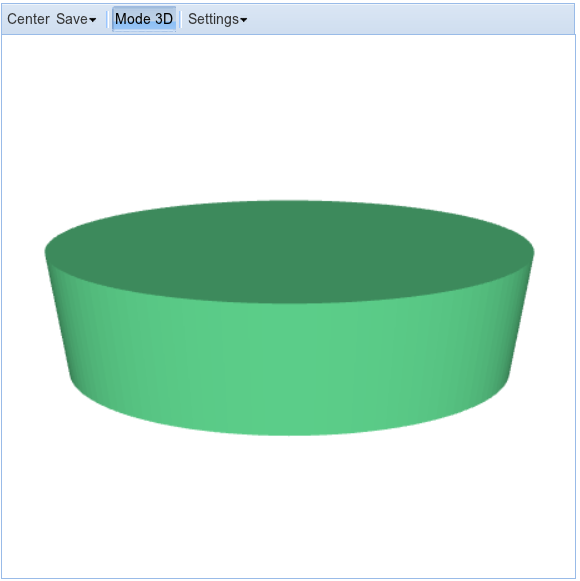
\includegraphics[width=0.5\textwidth]{img/scale-4.png}
\end{center}
\vspace{-2mm}
\caption{Cylinder scaled in the first and third axial directions by 2.0 and 4.0, respectively.}
\label{fig:scale-4}
%\vspace{-1cm}
\end{figure}
\noindent
Similarly, we could scale the object in the $xy$-plane using 

\begin{verbatim}
cyl4 = SCALE([1, 2])([2.0, 4.0])(cyl)
lab.view(cyl4, [0.4, 0.9, 0.6])
\end{verbatim}
or in the $yz$-plane using 

\begin{verbatim}
cyl4 = SCALE([2, 3])([2.0, 4.0])(cyl)
lab.view(cyl4, [0.4, 0.9, 0.6])
\end{verbatim}

\noindent
\underline{\em Scaling in all exial directions simultaneously}\\

The following command will 
scale the cylinder simultaneously in all three axial directions by the factors
2.0, 0.5 and 4.0.

\begin{verbatim}
cyl5 = SCALE([1, 2, 3])([2.0, 0.5, 4.0])(cyl)
lab.view(cyl5, [0.4, 0.9, 0.6])
\end{verbatim}
The output is shown in Fig. \ref{fig:scale-5}.

\newpage

\begin{figure}[!ht]
\begin{center}
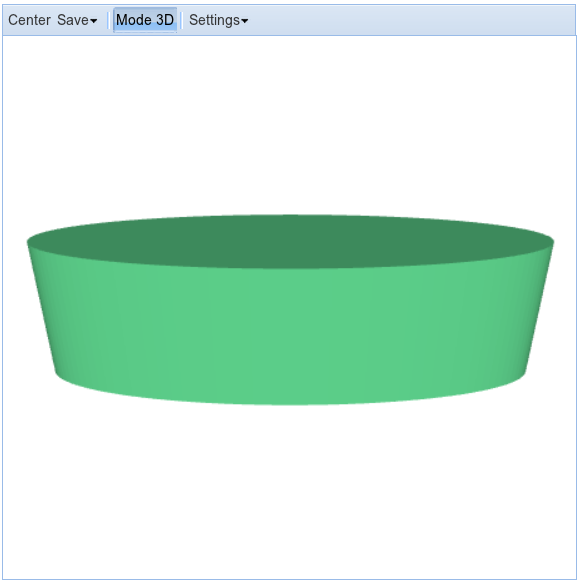
\includegraphics[width=0.5\textwidth]{img/scale-5.png}
\end{center}
\vspace{-2mm}
\caption{Cylinder scaled in all three axial directions simultaneously.}
\label{fig:scale-5}
%\vspace{-1cm}
\end{figure}
\noindent
We believe that the reader has now a good understanding of scaling.
In Section \ref{sec:translate} we will discuss in more detail how
to properly combine scaling with translations. 

\subsection{Enlarging an object}
If we want to just enlarge an object, we use the command SCALE and 
apply the same factor in all spatial directions. For example, to 
make a cylinder {\tt cyl} 5-times larger, we type:

\begin{verbatim}
cyl6 = SCALE([1, 2, 3])([5.0, 5.0, 5.0])(cyl)
lab.view(cyl6, [0.4, 0.9, 0.6])
\end{verbatim}


\subsection{Command TRANSLATE} \label{sec:translate}

The TRANSLATE command (abbreviated as T) can be used to move any 
object to a desired location. It takes three arguments: Axial directions,
displacements in these directions, and the object to be moved. For example,
the following program creates a unit cube and moves it by 1.5 in the 
$x$-direction:

\begin{verbatim}
from pyplasm import *
cube = CUBOID([1, 1, 1])
cube2 = T(1)(1.5)(cube)
\end{verbatim}
Another example: We create a unit sphere and move it simultaneously 
in the $x$-direction by 1.0 and in the $y$-direction by 2.0:

\begin{verbatim}
from pyplasm import *
s = SPHERE(1.0)([64, 64])
s2 = T([1, 2])([1.0, 2.0])(s)
\end{verbatim}
And last example: We create a unit sphere and  
move it simultaneously by -1.0 in the $x$-direction, by 1.0 in the $y$-direction
and by 4.0 in the $z$-direction:

\begin{verbatim}
from pyplasm import *
s = SPHERE(1.0)([64, 64])
s2 = T([1, 2, 3])([-1.0, 1.0, 4.0])(s)
\end{verbatim}

\subsection{Compound objects - command STRUCT}

Creating compound objects is necessary
for plotting multiple objects, since {\tt lab.view()} only can 
display a single object. This is also practical 
when we need to scale, translate, or rotate multiple objects at
once. For example, let's create a cube with a sphere on top of it.
It is always important to remember how a newly created
object is positioned in the global coordinate system. Concretely,
recall that 
a CUBOID is aligned with the axes as shown in Fig. \ref{fig:cuboid-1}

\begin{verbatim}
from pyplasm import *
color = [0.9, 0.9, 0.9]
c = CUBOID([2, 2, 2])
c2 = T([1, 2, 3])([1.0, 1.0, 2.0])(c)
c3 = T([1, 2, 3])([1.0, 1.0, 2.0])(c2)
\end{verbatim}
The way to display the three cubes together
is to create a compound object containing all of them:

\begin{verbatim}
comp = STRUCT([c, c2, c3])
lab.view(comp, [0.4, 0.9, 0.6])
\end{verbatim}
The output is shown in Fig. \ref{fig:comp-1}

\newpage

\begin{figure}[!ht]
\begin{center}
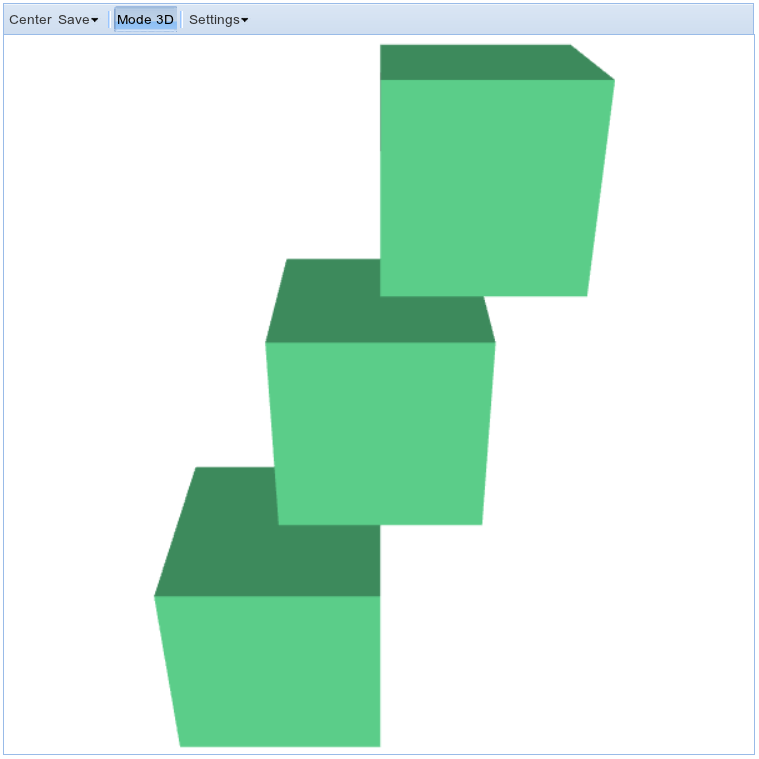
\includegraphics[width=0.5\textwidth]{img/comp-1.png}
\end{center}
\vspace{-2mm}
\caption{The way to display all cubes together is to use the STRUCT command.}
\label{fig:comp-1}
%\vspace{-1cm}
\end{figure}


\subsection{Putting objects on top of each other - command TOP}

The TOP command is a special case of translation that is very 
useful when we need to put objects on top of each other.
For illustration, let us put a sphere on top of a cube:

\begin{verbatim}
from pyplasm import *
c = CUBOID([2, 2, 2])
s = SPHERE(1.0)([64, 64])
lab.view(TOP([c, s]), color)
\end{verbatim}
The output is shown in Fig. \ref{fig:top-1}:

\newpage

\begin{figure}[!ht]
\begin{center}
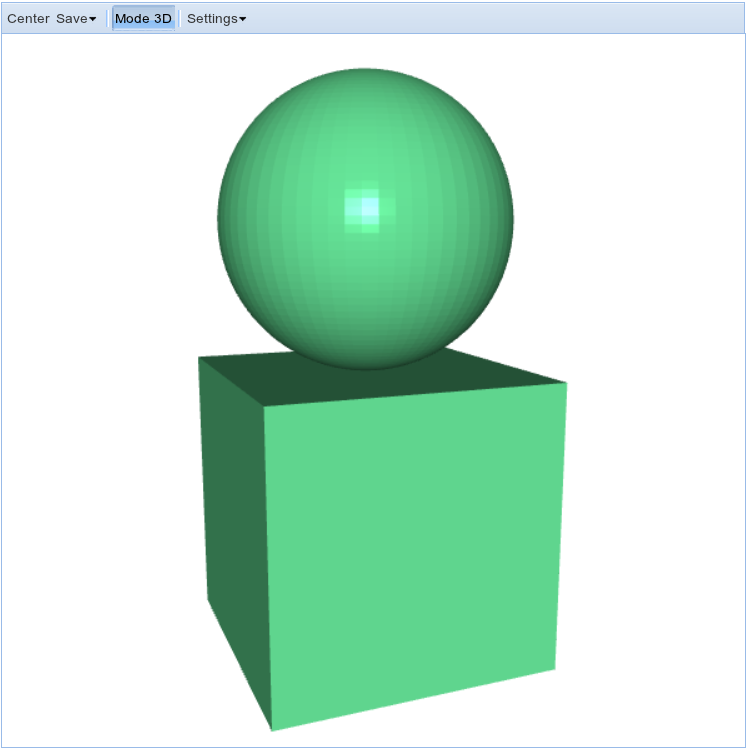
\includegraphics[width=0.5\textwidth]{img/top-1.png}
\end{center}
\vspace{-2mm}
\caption{Putting a sphere on top of a cube.}
\label{fig:top-1}
%\vspace{-1cm}
\end{figure}



\subsection{Command ROTATE}

Objects can be rotated using the command ROTATE (that
can be abbreviated as R). It has three parameters:
A pair of axes defining the plane of rotation (as integers),
an angle, and the object to be rotated. The axis of rotation 
always passes through the origin $[0, 0, 0]$, so it is important 
to know exactly where your object is located. 

For example, when creating 
a CUBOID, it is positioned as shown in Fig. \ref{fig:cuboid-1}.
Hence, the axis of rotation does not pass through its center!
This is best illustrated using a simple example. Let us create 
a unit cube, rotate it by $\pi$ (180 degrees), and display 
the rotated cube together with the original one:

\begin{verbatim}
from pyplasm import *
cube = CUBOID([1, 1, 1])
cube2 = R([1, 2])(PI)(cube)
comp = STRUCT([cube, cube2])
lab.view(comp, [0.4, 0.9, 0.6])
\end{verbatim}
The output is shown in Fig. \ref{fig:rot-1}.

\newpage

\begin{figure}[!ht]
\begin{center}
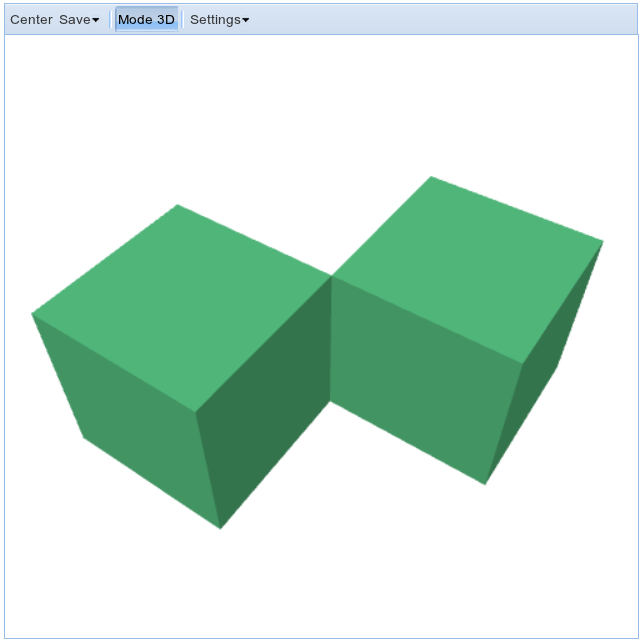
\includegraphics[width=0.5\textwidth]{img/rot-1.png}
\end{center}
\vspace{-2mm}
\caption{Unit cube rotated by $\pi$ (180 degrees) shown together with the original unit cube.}
\label{fig:rot-1}
%\vspace{-1cm}
\end{figure}
\noindent
In Fig. \ref{fig:rot-1}, the axis of rotation is where the two cubes meet. 

If we wanted to 
rotate the cube "in place", so that its center would not be moved,
we would have to first translate the cube in such a way that its center
lies at the origin. Let's do this. After moving the cube so that 
its center is at $[0, 0, 0]$, we will rotate it in two different directions,
then move it by 2.0 in the $x$-direction and display along with 
the original cube for comparison:

\begin{verbatim}
from pyplasm import *
cube = CUBOID([1, 1, 1])
cube2 = T([1, 2, 3])([-0.5, -0.5, -0.5])(cube)
cube3 = R([1, 2])(PI/4)(cube2)
cube4 = R([2, 3])(PI/4)(cube3)
cube5 = T(1)(2.0)(cube4)
comp = STRUCT([cube, cube5])
lab.view(comp, [0.4, 0.9, 0.6])
\end{verbatim}
The output is shown in Fig. \ref{fig:rot-2}.
\newpage

\begin{figure}[!ht]
\begin{center}
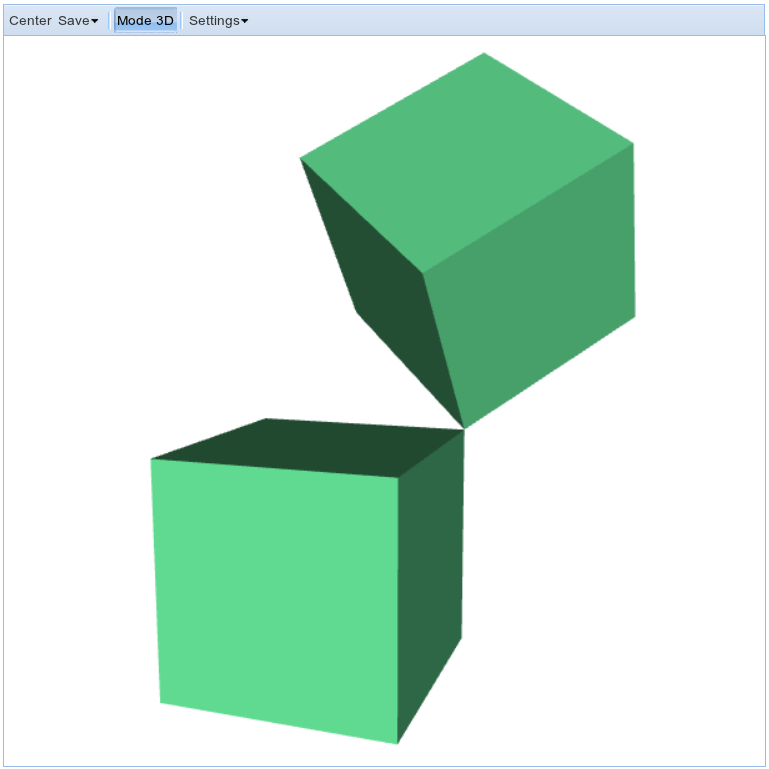
\includegraphics[width=0.5\textwidth]{img/rot-2.png}
\end{center}
\vspace{-2mm}
\caption{Cube rotated in two directions, then moved and shown along with the original cube.}
\label{fig:rot-2}
%\vspace{-1cm}
\end{figure}

\subsection{Exercises}

Coming soon.

\section{Binary Operations with Objects}

This is where things start to be real fun. Let us start with the 
command DIFF that makes it possible to drill holes, cut and slice objects, 
round edges, make imprints, and much more.

\subsection{Subtracting objects -- command DIFF}

The command DIFF makes it possible to subtract one object from another.
For illustration, we will create a $2 \times 2 \times 2$ cube and subtract 
a cylinder of radius 1.5 from it. It is important to remember where in the 
coordinate system the objects are created -- the cube lies in the 
first quadrant, with three of its edges meeting at the origin $[0, 0, 0]$.
The cylinder's axis coincides with the $z$-axis and the center of its base
circle is the origin. 

\begin{verbatim}
from pyplasm import *
c = CUBOID([2, 2, 2])
s = CYLINDER([1.5, 2])(128)
lab.view(DIFF([c, s]), [0.4, 0.9, 0.6]) 
\end{verbatim}
The output is shown in Fig. \ref{fig:diff-1}.

\newpage

\begin{figure}[!ht]
\begin{center}
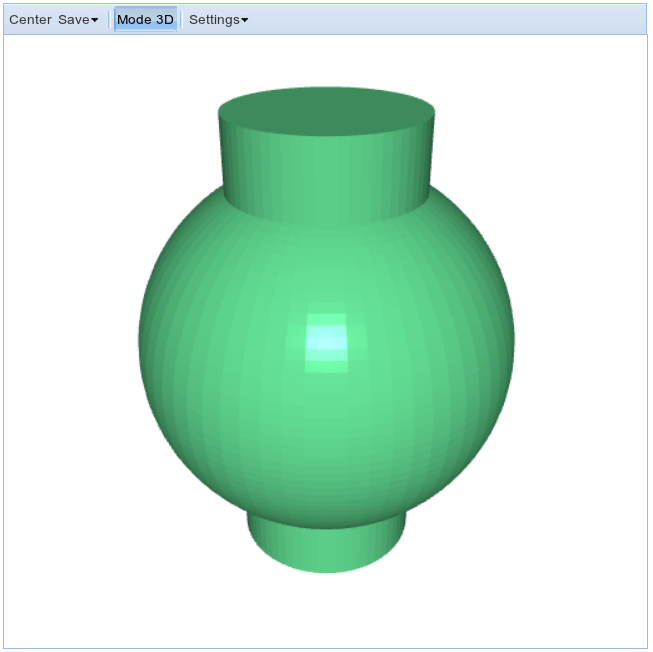
\includegraphics[width=0.5\textwidth]{img/diff-1.png}
\end{center}
\vspace{-2mm}
\caption{Subtracting the cylinder from the cube.}
\label{fig:diff-1}
%\vspace{-1cm}
\end{figure}
\noindent
We can also subtract the cube from the cylinder:

\begin{verbatim}
lab.view(DIFF([s, c]), [0.4, 0.9, 0.6]) 
\end{verbatim}
The output is shown in Fig. \ref{fig:diff-2}.

\newpage

\begin{figure}[!ht]
\begin{center}
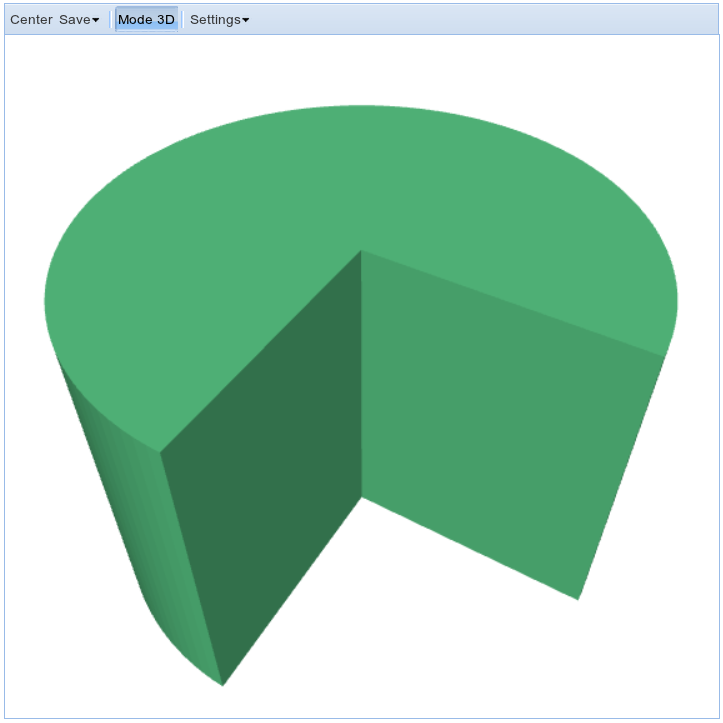
\includegraphics[width=0.5\textwidth]{img/diff-2.png}
\end{center}
\vspace{-2mm}
\caption{Subtracting the cube from the cylinder.}
\label{fig:diff-2}
%\vspace{-1cm}
\end{figure}
\noindent

\subsection{Surfaces and Solids -- command JOIN}

Some objects are solids (CUBOID, SPHERE) while others are surfaces (SPHERE, TORUS). 
Attempting to perform any binary operation (DIFF, UNION, INTERSECTION, ...) between
a solid and a surface will result into an error. This can be circumvented by 
converting the surface into a solid first, using the command JOIN. For example,
the following program will not work:

\begin{verbatim}
from pyplasm import *
c = CUBOID([2, 2, 2])
s = SPHERE(1.5)([64, 64])
lab.view(DIFF([c, s]), [0.9, 0.9, 0.9])
\end{verbatim}
but this program is correct:

\begin{verbatim}
from pyplasm import *
c = CUBOID([2, 2, 2])
s = JOIN(SPHERE(1.5)([64, 64]))
lab.view(DIFF([c, s]), [0.9, 0.9, 0.9])
\end{verbatim}




\subsection{Command UNION}

The UNION command creates a new object that is the set union 
of two or more objects. For simplicity, let us use the same objects
as in the previous example. 

\begin{verbatim}
from pyplasm import *
c = CUBOID([2, 2, 2])
s = CYLINDER([1.5, 2])(128)
lab.view(UNION([c, s]), [0.4, 0.9, 0.6]) 
\end{verbatim}
The output is shown in Fig. \ref{fig:union}.

%\newpage

\begin{figure}[!ht]
\begin{center}
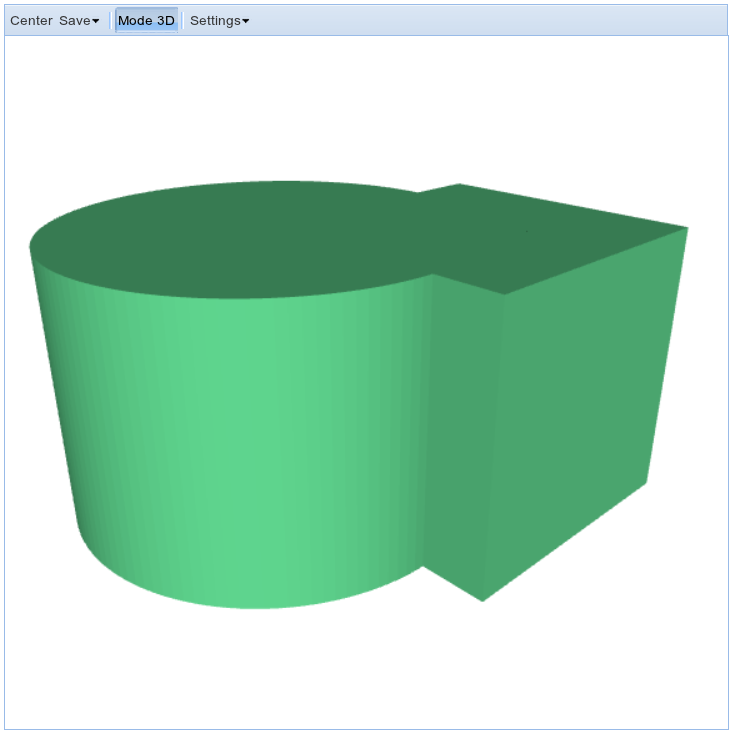
\includegraphics[width=0.5\textwidth]{img/union.png}
\end{center}
\vspace{-2mm}
\caption{Union of the cylinder and the cube.}
\label{fig:union}
%\vspace{-1cm}
\end{figure}


\subsection{Command INTERSECTION}

We will do two examples. First, for simplicity, we will create the intersection
of the cube and the cylinder from the previous paragraph:
 
\begin{verbatim}
from pyplasm import *
c = CUBOID([2, 2, 2])
s = CYLINDER([1.5, 2])(128)
lab.view(INTERSECTION([c, s]), [0.4, 0.9, 0.6]) 
\end{verbatim}
The output is shown in Fig. \ref{fig:int-2}.

\newpage

\begin{figure}[!ht]
\begin{center}
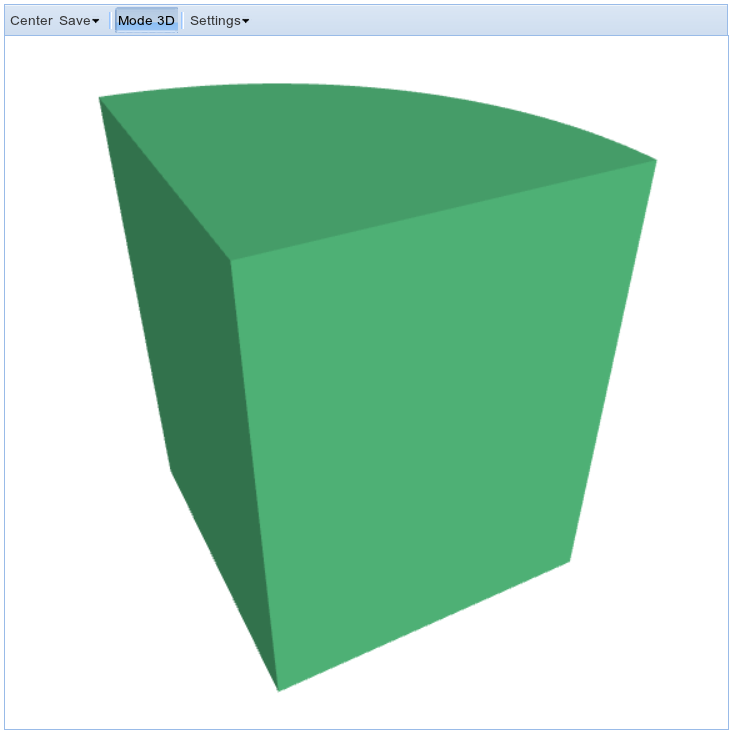
\includegraphics[width=0.5\textwidth]{img/int-2.png}
\end{center}
\vspace{-2mm}
\caption{Intersection of the cylinder and the cube.}
\label{fig:int-2}
%\vspace{-1cm}
\end{figure}
\noindent
In the second example, we will use the INTERSECTION command to create 
a strange object that looks link a square when viewed
from one direction, like a circle when viewed from another direction, 
and as a triangle when viewed from the third direction!


\begin{verbatim}
from pyplasm import *
color = [0.4, 0.9, 0.6]

# Cube.
c = CUBOID([2, 2, 2])
c = T([1, 2, 3])([-1, -1, -1])(c)

# Cylinder.
cyl = CYLINDER([1, 2])(64)
cyl = T([3])([-1])(cyl)

# Prism.
p = CONVEXHULL([[1, -1, -1], [1, 0, 1], [1, 1, -1], \
[-1, -1, -1], [-1, 0, 1], [-1, 1, -1]])

# Show their intersection.
lab.view(INTERSECTION([c, cyl, p]), color)
\end{verbatim}
The output is shown in Fig. \ref{fig:diff-1}.

\begin{figure}[!ht]
\begin{center}

\includegraphics[width=0.25\textwidth]{img/int-1a.png}
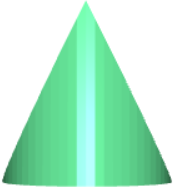
\includegraphics[width=0.25\textwidth]{img/int-1b.png}

\includegraphics[width=0.25\textwidth]{img/int-1c.png}
\end{center}
\vspace{-2mm}
\caption{Strange object!}
\label{fig:int-1}
%\vspace{-1cm}
\end{figure}


\subsection{Command XOR}

The operation XOR (exclusive logical OR) is "union minus intersection". Let us illustrate it 
on an example where we create a cube, and move it so that its center lies on the $z$-axis. Then 
we create a second cube by rotating the original cube by 45 degrees in the $xy$-plane. Last,
we XOR the two cubes. The corresponding code reads:
 
\begin{verbatim}
from pyplasm import *
color = [0.9, 0.9, 0.9]
c = CUBOID([2, 2, 2])
c = T([1, 2])([-1, -1])(c)
c2 = R([1, 2])(PI/4.)(c)
lab.view(XOR([c, c2]), color) 
\end{verbatim}
The output is shown in Fig. \ref{fig:xor-1}.

\newpage

\begin{figure}[!ht]
\begin{center}
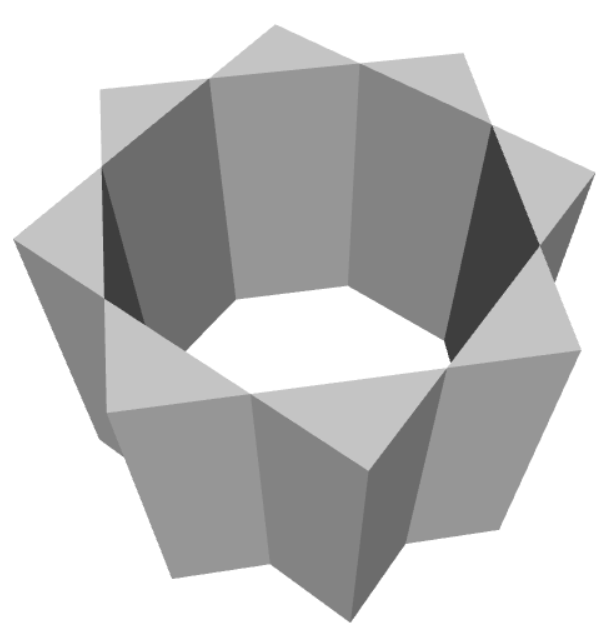
\includegraphics[width=0.5\textwidth]{img/xor-1.png}
\end{center}
\vspace{-2mm}
\caption{XOR of two overlapping cubes.}
\label{fig:xor-1}
%\vspace{-1cm}
\end{figure}
\noindent

\subsection{Exercises}

Solutions to all exercises from this section are available in the Solution Manual, and 
they can be also cloned in NCLab through Project $\rightarrow$ Clone in the 
File Manager's menu.\\

\noindent
\underline{\em Exercise C1: Ashtray}

Build a simple model of an ashtray using cylindrical shapes, 
as illustrated in Fig. \ref{fig:ashtray}.
All measures should be variable.

%\newpage

\begin{figure}[!ht]
\begin{center}
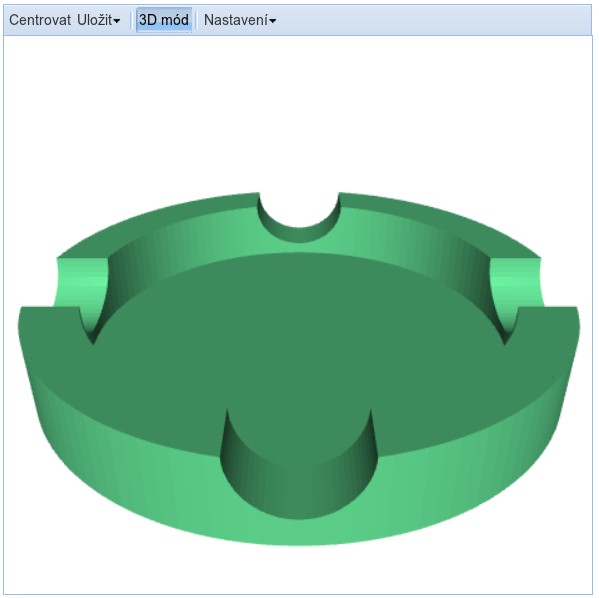
\includegraphics[width=0.5\textwidth]{img/ashtray.png}
\end{center}
\vspace{-2mm}
\caption{Illustration for Exercise C1.}
\label{fig:ashtray}
%\vspace{-1cm}
\end{figure}
\noindent
\noindent
\underline{\em Exercise C2: Drilled Cube}

Create a cube and drill three holes into it from the three axial 
directions, as illustrated in Fig. \ref{fig:drilledcube}.
The size of the cube as well as the diameter of the holes should 
be variable. 

%\newpage

\begin{figure}[!ht]
\begin{center}
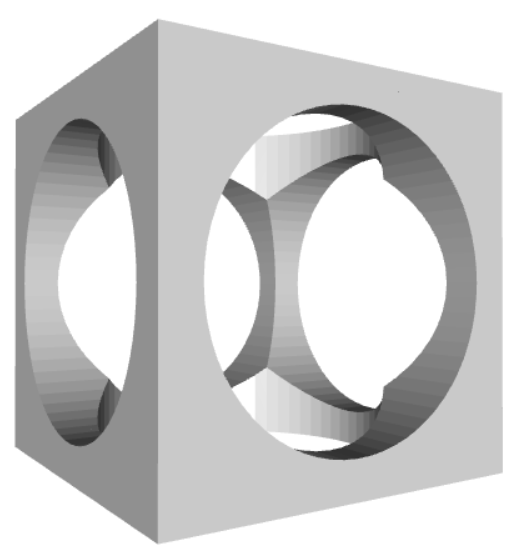
\includegraphics[width=0.5\textwidth]{img/drilledcube.png}
\end{center}
\vspace{-2mm}
\caption{Illustration for exercise C2.}
\label{fig:drilledcube}
%\vspace{-1cm}
\end{figure}
\noindent

\section{Creating Simple Objects (Continued)}

\subsection{Command STAR}

The STAR command will render a star with $N$ vertices. It is used as follows:
\begin{verbatim}
from pyplasm import *
N = 5
s = STAR(N)
lab.view(s, [0.4, 0.9, 0.6])
\end{verbatim}
The center of the star is at (0, 0), it is inscribed into the unit circle,  
and it lies in the $xy$-plane. Soon we will learn how to enlarge it, rotate it,
and translate it. The
output of the above code is shown in Fig. \ref{fig:star-1}.

\newpage

\begin{figure}[!ht]
\begin{center}
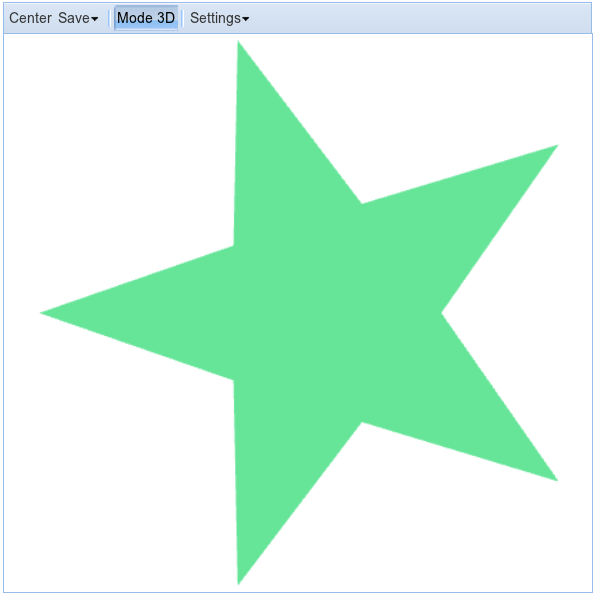
\includegraphics[width=0.5\textwidth]{img/star-1.png}
\end{center}
\vspace{-2mm}
\caption{Star with $N$ vertices inscribed into the unit circle.}
\label{fig:star-1}
%\vspace{-1cm}
\end{figure}

\subsection{Extrusion of 2D objects to 3D -- command POWER}

Any 2D object can be easily extruded into 3D, by performing 
Cartesian product with a 1D interval in the third direction. This 
is done using the POWER command. For example, the following code will
extrude the star that we created with the last program:

\begin{verbatim}
from pyplasm import *
N = 5
H = 1.0
s = STAR(N)
s3d = POWER([s, QUOTE([0, H])])
lab.view(s3d, [0.4, 0.9, 0.6])
\end{verbatim}
The command {\tt QUOTE([0, H])} creates an interval $(0, H)$. 
The output is displayed in Fig. \ref{fig:star-2}.

\newpage

\begin{figure}[!ht]
\begin{center}
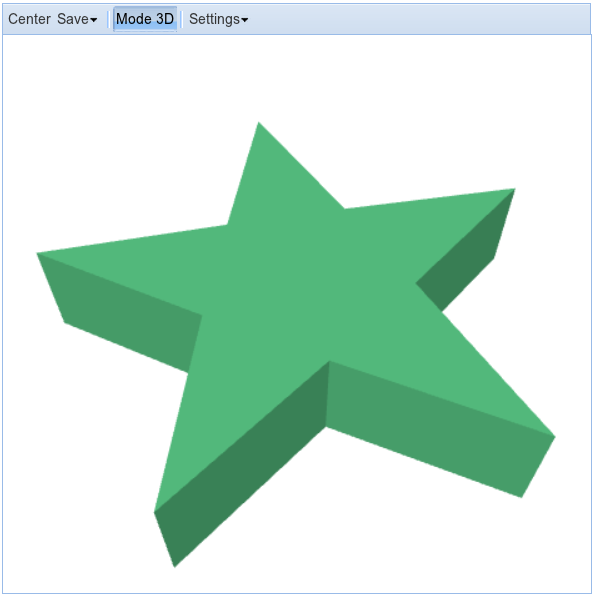
\includegraphics[width=0.5\textwidth]{img/star-2.png}
\end{center}
\vspace{-2mm}
\caption{3D star obtained from the original 2D star via the QUOTE and POWER commands.}
\label{fig:star-2}
%\vspace{-1cm}
\end{figure}

\subsection{General polygons and polyhedra -- command MKPOL}

Coming soon.

\subsection{Extracting boundary vertices, edges and faces -- command SKELETON}

Coming soon.



\section{Curves and Curved Surfaces}

Coming soon.

\section{The Power of Scripting}

The fact that PLaSM functions are accessible from withing the Python 
interpreter gives us significant additional power to automate things 
-- we can create objects that would be too complicated to create manually. 
Let us see an example of this.

\subsection{Intersection of $N$ randomly generated cubes}

The title says it all. We are calculating the intersection of 
$N$ cubes that have the same size, same center, and they are 
randomly rotated. For the purposes of this calculation, we
set $N = 100$:

{\small
\begin{verbatim}
# Import libraries.
from pyplasm import *
from numpy import *

# Define 'n' random rotations.
def randRots(n):
    v = random.random_sample(4*n)
    return [ [2*PI*v[i],[v[i+1],v[i+2],v[i+3]]] for i in range(0,4*n,4) ]

# Number of cubes to intersect.
N = 100
  
# Intersect N randomly rotated cubes.
Cube = T([1, 2, 3])([-1, -1, -1])(CUBOID([2, 2, 2]))
rotations = AA(ROTN)(randRots(N))
out = TREE(COMP([JOIN, INTERSECTION]))(CONS(rotations)(Cube))

# View the result. The numbers between 0 and 1 
# are RGB components.
lab.view(out, [0.4, 0.9, 0.6])
\end{verbatim}
}
\noindent
The corresponding output is shown in Fig. \ref{fig:random_cubes}.

\newpage

\begin{figure}[!ht]
\begin{center}
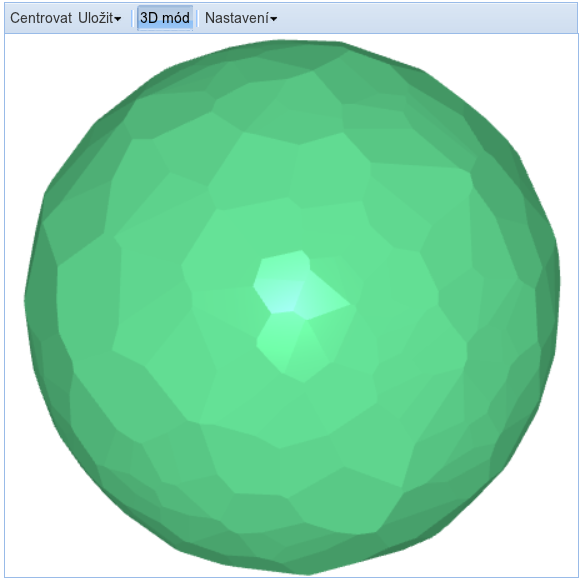
\includegraphics[width=0.5\textwidth]{img/random_cubes.png}
\end{center}
\vspace{-2mm}
\caption{Intersection of 100 randomly rotated cubes.}
\label{fig:random_cubes}
%\vspace{-1cm}
\end{figure}
\noindent





\subsection{Exercises}

Solutions to all exercises from this section are available in the Solution Manual, and 
they can also be cloned in NCLab through Project $\rightarrow$ Clone in the 
File Manager's menu.\\

\noindent
\underline{\em Exercise D1: Aztec Pyramid}

Build an Aztec Pyramid as illustrated in Fig. \ref{fig:aztec}. The length 
on the base edge, length of the top edge, height, and the number of layers
should be user-defined parameters. 

\newpage

\begin{figure}[!ht]
\begin{center}
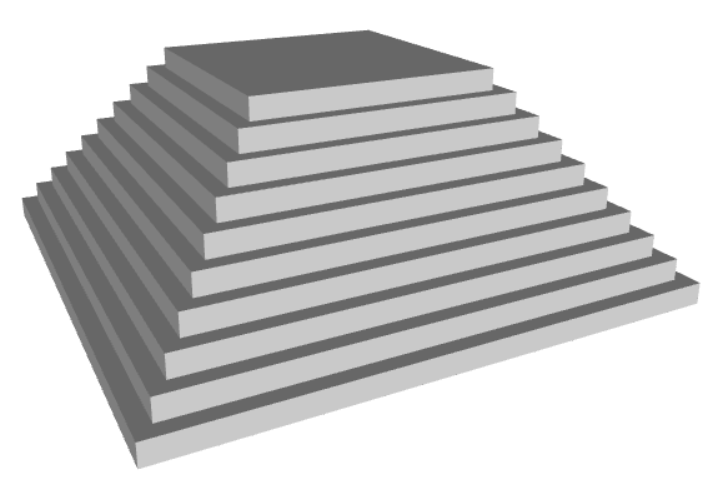
\includegraphics[width=0.7\textwidth]{img/aztec.png}
\end{center}
\vspace{-2mm}
\caption{Illustration for exercise D1.}
\label{fig:aztec}
%\vspace{-1cm}
\end{figure}
\noindent

\noindent
\underline{\em Exercise D2: Tower of Hanoi}

Build a model of the Tower of Hanoi game as illustrated in Fig. \ref{fig:hanoi}. 
The radius of the largest and smallest disc, and the height of the tower 
should be user-defined parameters. 

%\newpage

\begin{figure}[!ht]
\begin{center}
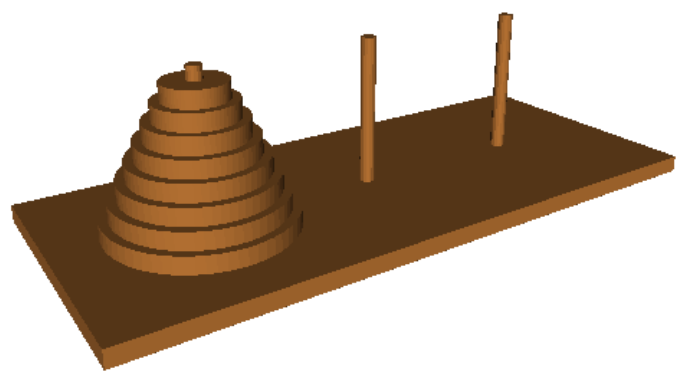
\includegraphics[width=0.7\textwidth]{img/hanoi.png}
\end{center}
\vspace{-2mm}
\caption{Illustration for exercise D2.}
\label{fig:hanoi}
%\vspace{-1cm}
\end{figure}
\noindent

\newpage


\noindent
\underline{\em Exercise 3: Horse Corral}

Build a corral for horses with variable radius $r$ and variable number 
of equally-long sides $N$. Also the vertical poles should have general user-defined 
dimensions $W \times W \times H$. Illustrative images of how the corral should look like 
are shown in Fig. \ref{fig:corral2}.

\begin{figure}[!ht]
\begin{center}
\includegraphics[width=0.5\textwidth]{img/tam-3.png}
\end{center}
\vspace{-2mm}
\caption{Illustration for exercise D3.}
\label{fig:corral2}
%\vspace{-1cm}
\end{figure}
\noindent

\noindent
\underline{\em Exercise D4: Wagon Wheel}

Build a spoked wagon wheel similar to the one in Fig. \ref{fig:wheel-1}. All radiuses 
and thicknesses should be user-defined, as well as the number of spokes.

\begin{figure}[!ht]
\begin{center}
\includegraphics[width=0.5\textwidth]{img/wagonwheel-1.png}
\end{center}
\vspace{-2mm}
\caption{Illustration for exercise D4.}
\label{fig:wheel-1}
%\vspace{-1cm}
\end{figure}
\noindent



\section{Advanced Examples}

All examples in this section can be cloned in NCLab through 
Project $\rightarrow$ Clone in the File Manager's menu.

\subsection{Temple}

This example shows a model of a temple. Take some 
time to walk through it, you'll feel like in ancient Rome!
{\small
\begin{verbatim}
from pyplasm import *

def out():
    def Column (r,h):
        basis = CUBOID([ 2*r*1.2, 2*r*1.2, h/12.0 ]) 
        trunk = CYLINDER([ r, (10.0/12.0)*h ]) (36)
        capital = basis
        beam = S(1)(3)(capital) 
        return TOP([TOP([TOP([basis,trunk]),capital]),beam])
    def Gable (radius,h,n): 
        lastX = n*3*(2*radius*1.2)
        triangle = MKPOL([[[0,0],[lastX,0],[lastX/2.0,h/2]],[[1,2,3]],[[1]]])
        return R([2,3])(PI/2)(Plasm.power(triangle  , QUOTE([radius*1.2])  ))
    col = Column(1, 12)
    def ColRow (n): 
        return INSR(RIGHT)([col for i in range(n)])
    ColRowAndGable =  TOP([ColRow(4),Gable(1,12,4) ])
    Temple = STRUCT(  CAT([
        [ColRowAndGable, T(2)(6)], 
        DOUBLE_DIESIS(4)([  ColRow(4),T(2)(6)  ]), 
        [ColRowAndGable] 
        ]))
    Ground = EMBED(1)(BOX([1,2])(Temple))
    Xsizes = QUOTE( DOUBLE_DIESIS(14)([0.6,-1.2]) )
    Ysizes = QUOTE( AL([ -0.7, DOUBLE_DIESIS(5)([-1,5]) ]))
    Zsizes = QUOTE([ -13, 0.6 ])
    SecondaryBeams = Plasm.power(Plasm.power(Xsizes,Ysizes),Zsizes)
    return STRUCT([Temple, SecondaryBeams, Ground])

lab.view(out(), [0.9, 0.9, 0.9])
\end{verbatim}
}
\noindent
The corresponding output is shown in Fig. \ref{fig:temple}.

\begin{figure}[!ht]
\begin{center}
\includegraphics[width=0.8\textwidth]{img/temple.png}
\end{center}
\vspace{-2mm}
\caption{Temple.}
\label{fig:temple}
%\vspace{-1cm}
\end{figure}
\noindent




\end{document}
